% !TEX TS-program = xelatex

%
%Не забыть:
%--------------------------------------
%Вставить колонтитулы, поменять название на титульнике



%--------------------------------------

\documentclass[a4paper, 9pt, twocolumn]{book} 

%--------------------------------------
%Part for XeLaTex for Russian language (delete in case using pdfLatex)
%--------------------------------------
% Languages.
\usepackage{polyglossia}
\RequirePackage{polyglossia}
\setdefaultlanguage{russian}
\setotherlanguage{english}

% Fonts.
\usepackage{fontspec}[Path=/Users/fess/Library/Fonts/]
\RequirePackage{fontspec}
\newfontfamily\russianfont[Ligatures=TeX]{Bookmania}
\newfontfamily\englishfont[Ligatures=TeX]{Bookmania}

%--------------------------------------
%Russian-specific packages
%--------------------------------------
%\usepackage[T2A]{fontenc}
%\usepackage[utf8]{inputenc}
%\usepackage[english,russian]{babel}
%\usepackage[intlimits]{amsmath}
%\usepackage{esint}
%--------------------------------------
%Hyphenation rules
%--------------------------------------
\usepackage{hyphenat}
\hyphenation{ма-те-ма-ти-ка вос-ста-нав-ли-ва-ть}
\hyphenation{предметов}
%--------------------------------------
%Packages
%--------------------------------------
\usepackage{amsmath}
\usepackage{amssymb}
\usepackage{amsfonts}
\usepackage{amsthm}
\usepackage{latexsym}
\usepackage{mathtools}
\usepackage{etoolbox}%Булевые операторы
\usepackage{extsizes}%Выставление произвольного шрифта в \documentclass
\usepackage{geometry}%Разметка листа
\usepackage{indentfirst}
\usepackage{wrapfig}%Создание обтекаемых текстом объектов
\usepackage{fancyhdr}%Создание колонтитулов
\usepackage{setspace}%Настройка интерлиньяжа
\usepackage{lastpage}%Вывод номера последней страницы в документе, \lastpage
\usepackage{soul}%Изменение параметров начертания
\usepackage{hyperref}%Две строчки с настройкой гиперссылок внутри получаеммого
\usepackage[usenames,dvipsnames,svgnames,table,rgb]{xcolor}% pdf-документа
\usepackage{multicol}%Позволяет писать текст в несколько колонок
\usepackage{cite}%Работа с библиографией
\usepackage{subfigure}% Человеческая вставка нескольких картинок
\usepackage{tikz}%Рисование рисунков
\usepackage{xcolor}%Возможность устанавливать цвет шрифта
\usepackage{float}% Возможность ставить H в положениях картинки
\usepackage{titlesec}% Дополнительные уровни section
% Настройка titlesec:
\titleformat{\paragraph}
{\normalfont\normalsize\bfseries}{\theparagraph}{1em}{}
\titlespacing*{\paragraph}
{0pt}{3.25ex plus 1ex minus .2ex}{1.5ex plus .2ex}
\setcounter{secnumdepth}{-1}
\setcounter{tocdepth}{4}
\titleformat*{\subsection}{\Large\bfseries}
% Настройка оглавления в 2 колонки
\usepackage[toc]{multitoc}
\renewcommand*{\multicolumntoc}{2}
%Настройка цветов секций и т.п.
\usepackage{sectsty}
\definecolor{sectioncolor}{RGB}{81, 28, 18}

\sectionfont{\color{sectioncolor}}
\subsectionfont{\color{sectioncolor}}
\subsubsectionfont{\color{sectioncolor}}


% Для картинок Моти
\usepackage{misccorr}
\usepackage{lscape}
\usepackage{cmap}



\usepackage{graphicx}
\graphicspath{{Pictures/}}
\DeclareGraphicsExtensions{.pdf,.png,.jpg}

\usepackage{eso-pic}

%\usepackage{background}
%\backgroundsetup{scale=1.2, angle=0, firstpage=true, opacity=1, contents={\begin{tikzpicture}[remember picture,overlay]
%		\node at([yshift=0pt, xshift=0pt]current page.center)
%		{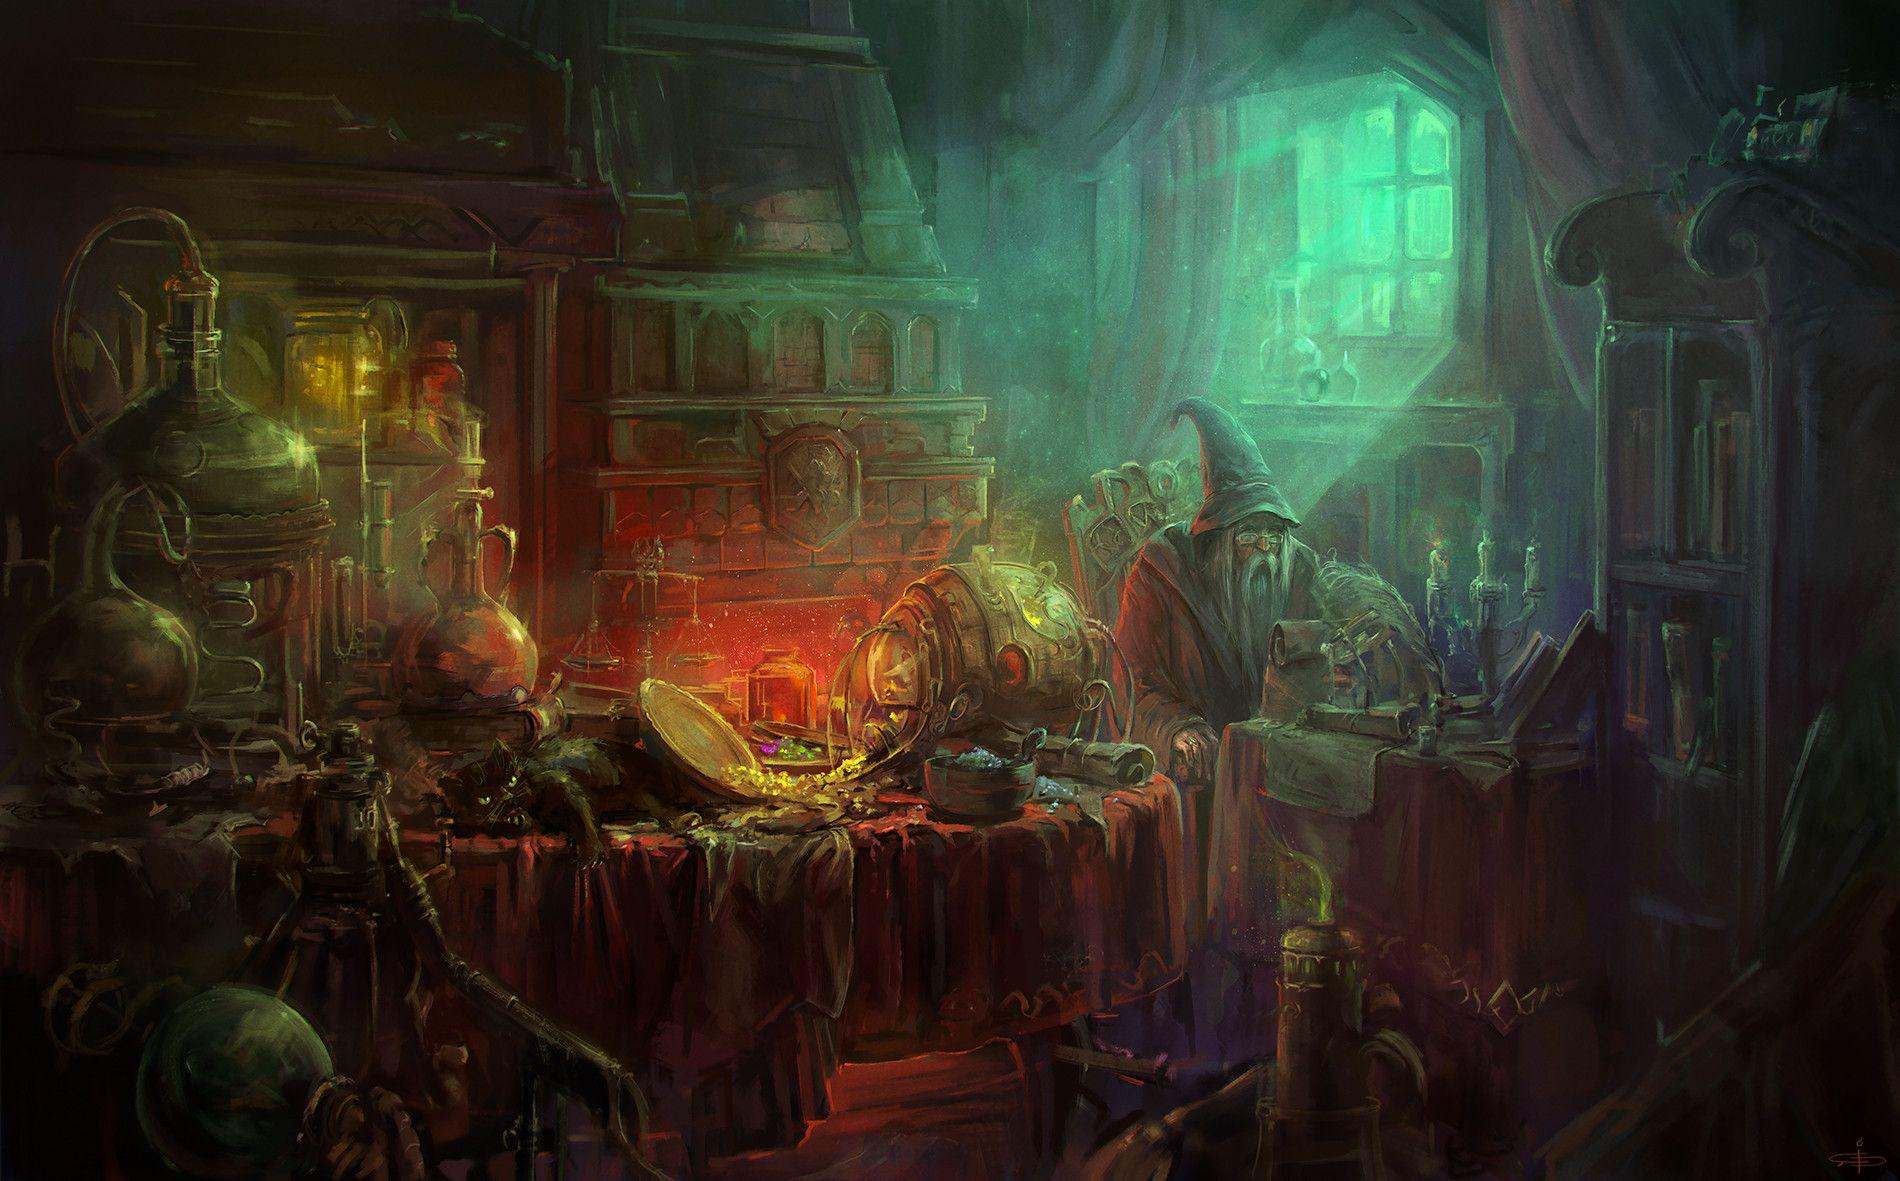
\includegraphics{Title}};
%		\end{tikzpicture}}}

%----------------------------------------
%Список окружений
%----------------------------------------
\newenvironment {theor}[2]
{\smallskip \par \textbf{#1.} \textit{#2}  \par $\blacktriangleleft$}
{\flushright{$\blacktriangleright$} \medskip \par} %лемма/теорема с доказательством
\newenvironment {proofn}
{\par $\blacktriangleleft$}
{$\blacktriangleright$ \par} %доказательство
%----------------------------------------
%Список команд
%----------------------------------------
\newcommand{\grad}
{\mathop{\mathrm{grad}}\nolimits\,} %градиент

\newcommand{\diver}
{\mathop{\mathrm{div}}\nolimits\,} %дивергенция

\newcommand{\rot}
{\ensuremath{\mathrm{rot}}\,}

\newcommand{\Def}[1]
{\underline{\textbf{#1}}} %определение

\newcommand{\RN}[1]
{\MakeUppercase{\romannumeral #1}} %римские цифры

\newcommand {\theornp}[2]
{\textbf{#1.} \textit{ #2} \par} %Написание леммы/теоремы без доказательства

\newcommand{\qrq}
{\ensuremath{\quad \Rightarrow \quad}} %Человеческий знак следствия

\newcommand{\qlrq}
{\ensuremath{\quad \Leftrightarrow \quad}} %Человеческий знак равносильности

\renewcommand{\phi}{\varphi} %Нормальный знак фи

\newcommand{\me}
{\ensuremath{\mathbb{E}}}

\newcommand{\md}
{\ensuremath{\mathbb{D}}}

\newcommand{\newsubsection}[1]{
	{\subsection{#1}}
	\vskip -0.45cm
	\noindent
	\rule{\linewidth}{1.8pt}
}




%\renewcommand{\vec}{\overline}




%----------------------------------------
%Разметка листа
%----------------------------------------
\geometry{top = 3cm}
\geometry{bottom = 2cm}
\geometry{left = 1.5cm}
\geometry{right = 1.5cm}
%----------------------------------------
%Колонтитулы
%----------------------------------------
\pagestyle{fancy}%Создание колонтитулов
\fancyhead{}
%\fancyfoot{}
\fancyhead[R]{\textsc{Уравнения Лондонов. Кинетическая индуктивность сверхпроводников.}}%Вставить колонтитул сюда
%----------------------------------------
%Интерлиньяж (расстояния между строчками)
%----------------------------------------
%\onehalfspacing -- интерлиньяж 1.5
%\doublespacing -- интерлиньяж 2
%----------------------------------------
%Настройка гиперссылок
%----------------------------------------
\hypersetup{				% Гиперссылки
	unicode=true,           % русские буквы в раздела PDF
	pdftitle={Заголовок},   % Заголовок
	pdfauthor={Автор},      % Автор
	pdfsubject={Тема},      % Тема
	pdfcreator={Создатель}, % Создатель
	pdfproducer={Производитель}, % Производитель
	pdfkeywords={keyword1} {key2} {key3}, % Ключевые слова
	colorlinks=true,       	% false: ссылки в рамках; true: цветные ссылки
	linkcolor=blue,          % внутренние ссылки
	citecolor=blue,        % на библиографию
	filecolor=magenta,      % на файлы
	urlcolor=red           % на URL
}
%----------------------------------------
%Работа с библиографией (как бич)
%----------------------------------------
%\renewcommand{\refname}{Список литературы}%Изменение названия списка литературы для article
%\renewcommand{\bibname}{Список литературы}%Изменение названия списка литературы для book и report
%----------------------------------------
\begin{document}
	\begin{titlepage}
		\AddToShipoutPictureBG*{%
			\put(0,0){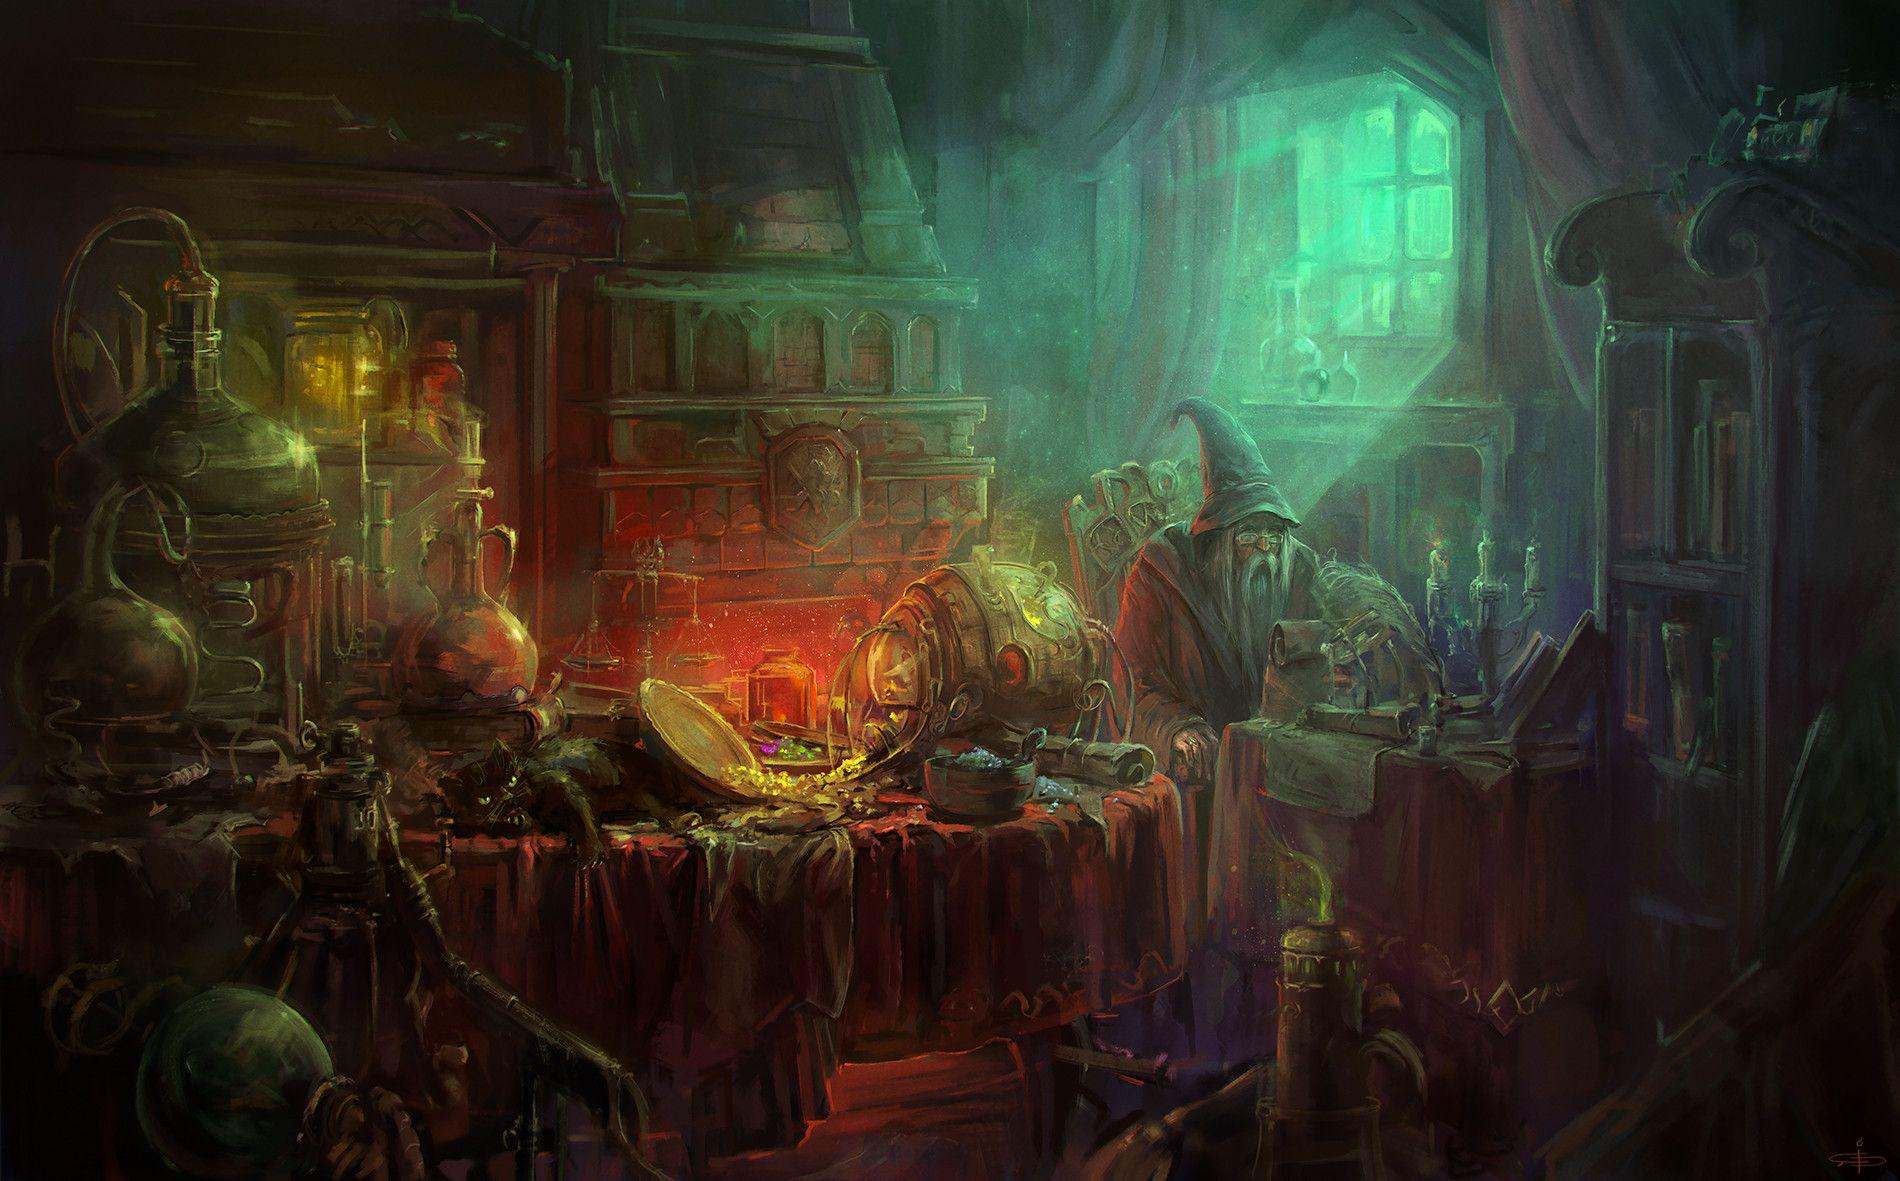
\includegraphics[scale=1.2]{Title}}%
		}
		\begin{center}
			\begin{figure}[H]
				\centering
				
\includegraphics[scale=0.2]{DnD_logo}
			\end{figure}
			{\fontsize{30pt}{0pt}\textcolor{white}{\textbf{Всеобъемлющее руководство по сбору и созданию предметов}}}
			
			\begin{figure}[H]
				\centering
				
\includegraphics[scale=0.2]{Arrow}
			\end{figure}			
			
				\vskip 13cm
				
			{\Large{\textcolor{white}{Руководство по системе сбора и создания предметов в одной из лучших ролевых игр мира}}}
			
		\end{center}
	\end{titlepage}

	\AddToShipoutPictureBG{%
		\put(0,0){
\includegraphics[scale=1.2]{Base}}%
	}

	\tableofcontents
	
	\chapter{Сбор материалов}
	
	\section{Травничество}
	
	Ремесло поиска, сбора и определения растений и ингредиентов для последующего их использования в алхимических субстанциях. Пока игроки путешествуют по миру, они могут захотеть взять с собой какие-то местные растения. Травничество используется для сбора таких вещей как лепестки, семена, корни, грибы, листья и много другое.
	
	Чтобы собирать ингредиенты, необходим набор травника, в котором есть ножницы и прочие инструменты для отделения необходимых частей растений. Для последующего хранения или продажи полученных ресурсов используются флаконы, мешочки и прочие контейнеры.
	
	Приведенное ниже руководство покажет вам три основных функции Травничества.
	
	\newsubsection{Поиск трав}
	
	Вы можете провести одну \textbf{проверку Мудрости (Природа/Набор травника) КС 15}, чтобы определить, можете ли вы найти что-то, что можно было бы собрать. Сравните полученный результат с таблицей \textbf{Сбор трав}, чтобы определить максимальное число \textbf{проверок Сбора}, которые вы можете совершить. Каждый отдельный сбор трав занимает \textbf{1 час}; вы не обязаны пользоваться всеми доступными проверками.
	
	Базовый КС составляет 15, однако, это значение может быть скорректировано (или проверка может вообще оказаться недоступной) в зависимости от окружающей среды. Например, если вы путешествуете через скалистые горы, растения могут быть редкими, или же могут вообще не расти на камнях.
	
	Если у вас есть владение набором травника, но нет владения навыком Природа, добавляйте бонус мастерства к проверкам. Если у вас есть владение и тем, и тем, вы получаете \textbf{преимущество} на эту проверку.
	
	\subsubsection*{Направленный поиск}
	
	Вероятно, вы наверняка знаете, что вы ищите. В качестве альтернативы обычной проверке, вы можете выбрать определенный известный ингредиент, который вы хотите найти в текущем биоме. Проведите проверку \textbf{Мудрости (Природа/Набор травника) КС 15 + модификатор КС ингредиента}. В случае провала, вы тратите 1 час и не находите искомый ингридиент. Если вы проводите поиск конкретного ингредиента, то вы можете провести сбор лишь один раз.
	
	\subsubsection*{Далекие путешествия}
	
	В течении светового дня вы можете углубляться в дикую природу, чтобы добираться до удаленных биомов. В зависимости от того, где в мире вы находитесь, вы можете предпринимать путешествия в далекие места при условии что у вас есть достаточно свободного времени чтобы туда дойти, собрать травы и вернуться назад. За каждый день, проведенный в поиске трав, вы можете совершить до двух проверок Травничества.
	
	\section{Сбор растений}
	
	\subsection{Проверка сбора}
	
	Вы успешно нашли растение. Теперь его необходимо собрать. Совершите \textbf{проверки сбора} в количестве вплоть до указанного в таблице \textbf{Сбор трав} значения совершая броски \textbf{1d2, 2d6 и 1d12} для каждого сбора. Каждый отдельный сбор занимает 1 час.
	
	Персонажи, имеющие владение набором травника, имеют большие навыки в сборе ингредиентов и получении бонусов при этом. Они получают +1 бонус к количеству получаемых при сборе ингредиентов при владении набора травника и +2 бонус при наличии \textbf{Компетентности} с ним. Рейнджеры и друиды также получают дополнительный +1 бонус в силу их единства с природой. Эти бонусы суммируются, поэтому рейнджер, имеющий владение набором травника, будет получать +2 ко всем проверкам Сбора при использовании 1d2. Это значит, что они всегда будут находить или извлекать как минимум 3 порции каждого из получаемых ингредиентов.
	
	\paragraph*{Тип ингредиента: 2d6}
	\noindent
	\begin{itemize}
		\item Данный бросок совершается по таблице, соответствующей местности (биому), в которой вы сейчас находитесь. Сравните полученный результат с ней, чтобы определить, какое растение вы обнаружили.
	\end{itemize}
	
	\paragraph*{Эффективность сбора: 1d2}
	
	\noindent\textit{(+1 для Рейнджеров и Друидов)}
	
	\noindent\textit{(+1 за владение набором травника и +2 за компетентность с ним)}
	\noindent
	\begin{itemize}
		\item Результат данного броска определяет, сколько порций обнаруженного растения вы можете получить при сборе. 
	\end{itemize}

	\paragraph*{Тип обычного ингредиента (совершается на всегда): 1d12}
	
	\begin{itemize}
		\item Этот бросок совершается в том случае, если при броске 2d6 вам выпало 6, 7 или 8. В таком случае в таблице текущего биома будет указано <<обычный ингредиент>>. Совершив бросок, обратитесь к таблице <<Обычные ингредиенты>>, чтобы узнать, какое растение вы обнаружили.
	\end{itemize}
	
	\paragraph*{Пример сбора:}
	
	Вы находитесь в лесу и ищете ингредиенты. При совершении бросков вы получили следующий результат:
	
	\begin{itemize}
		\item 1d2 = 2
		\item 2d6 = 4
		\item 1d12 --- не важен при результате на 2d6 меньше 6
	\end{itemize}

	Получается, что согласно таблице \textbf{Лес} вы получили 2 единицы рвоска.
	
	\section{Определение растений}
	
	\subsection{Неизвестные ингредиенты}
	
	Что происходит, если вы находите неизвестный вам до этого момента ингредиент? Проведите проверку \textbf{Интеллекта (Природа/набор травника)}, чтобы понять, можете ли вы определить, что это за растение и каковы его возможные полезные свойства (пассивные значения и предыдущие проверки могут давать автоматический успех). КС этого броска определяется как \textbf{15 + модификатор КС ингредиента}.
	
	Если у вас есть владение набором травника, но нет владения навыком Природа, добавляйте бонус мастерства к проверкам. Если у вас есть владение и тем, и тем, вы получаете \textbf{преимущество} на эту проверку.
	
	В случае успеха вы узнаете название растения и \textbf{формулу} для его использования в зелье или яде.
	
	%Пофиксить страницу
	
	Если у вас не получается определить ингредиент, то вы можете провести с этой целью исследование (XGE 132), или же провести эксперименты. Каждой единицы полученного ингредиента достаточно для проведения одной попытки эксперимента для определения его полезных свойств (см. раздел \textbf{Алхимия} ниже).
	
	\paragraph*{Ограничение на возможные знания}
	
	Вероятно, тот, с кем вы общаетесь, обладает ограниченным количеством информации. Это ограничение может проявляться тремя различными способами:
	
	\begin{itemize}
		\item \textbf{Экосистема} (лесные растения, горные, и т.д)
		
		\item \textbf{Редкость} (обычные, необычные, редкие или очень редкие)
		
		\item \textbf{Использование} (зелья или яды)
	\end{itemize}

	Алхимик или травник, с которым вы общаетесь, может, к примеру, заниматься только зельями, или же может быть ограничен знанием исключительно тех ингредиентов, которые произрастают неподалеку.	
	
	\section{Продажа трав}
	
	Травы и обычные растения зачастую продаются в больших и не очень городах, а иногда и в деревнях. Это может происходить либо днем, либо только в определенные периоды, однако способ торговли от этого не зависит. Однако, в зависимости от экономики вашего мира, цены и количество продаваемых ингредиентов может разительно отличаться.
	
	Не ожидайте, что вы придете в город Вилсбури, который недавно был ограблен орками, и продадите ваши запасы трав по лучшей цене. Вряд ли у вас вообще это получится. Иногда вам может повезти и вы продадите все ненужные ингредиенты в столице, которая всегда нуждается в свежих травах, иногда же вам придется припрятать ваши запасы на некоторое время.
	
	Если рассматривать обычные ежедневные обстоятельства, то игрок может продать пригоршню или две обычных ингредиентов торговцу в большом или не очень городе. Однако сумма денег, получаемая за эту сделку, может все равно сильно варьироваться. Редкие ингредиенты обычно тяжело продать за полную цену, а вообще найти для них покупателя обычно еще сложнее.
	
	Как и при продаже магических предметов, игроку необходимо провести проверку \textbf{Интеллекта (Анализ) КС 20}, чтобы найти потенциальных покупателей для их товаров. Другой игрок в группе может помочь в этом непростом деле, предлагая услуги сотоварища, даруя при этом первому игроку преимущество на этот бросок.
	
	В случае провала, покупатель не находится до тех пор, пока игрок не совершит длительный отдых и не предпримет еще одну попытку. В случае успеха, игрок  находит покупателя неподалеку. Если это произошло во время простоя, то для этого должно пройти время, определяемое  редкостью ингредиента. Кроме того, она же может повлиять на вероятность того, что цена окажется не максимальной для отдельно взятого ингредиента. Обратитесь к таблице ниже, чтобы определить как цены, предлагаемые покупателем, так и необходимое число дней да его нахождения.
	
	\textbf{Продажа трав}
	
	\begin{center}
		
		\begin{tabular}{|c|c|c|c|}
			\hline
			\textbf{Редкость} & \textbf{Цена} & \textbf{Модификатор d100} & \textbf{Дней чтобы найти покупателя (шанс за день)} \\
			\hline
			Обычный & До 15 зм & +10 & 1d4 (25\% за один день) \\
			\hline
			Необычный & 16--40 зм & +0 & 1d6 (17\% за один день) \\
			\hline
			Редкий & 41--100 зм & -10 & 1d8 (13\% за один день) \\
			\hline
			Очень редкий & 100+ зм & -20 & 1d10 (10\% за один день) \\
			\hline
		\end{tabular}
		
	\end{center}

	Модификатор d100 прибавляется к броску по таблице ниже.
	
	\medspace

	\textbf{Цены трав}
	
	\begin{center}
		
		\begin{tabular}{|c|l|}
			\hline
			\textbf{d100 + модификатор} & \textbf{Вы находите...} \\
			\hline
			20 или меньше & Покупатель предлагает десятую часть базовой цены \\
			\hline
			21--40 & Покупатель предлагает пятую часть базовой цены. Сомнительный покупатель предлагает половину базовой цены \\
			\hline
			41--80 & Покупатель предлагает половину базовой цены. Сомнительный предлагает полную цену \\
			\hline
			81--90 & Покупатель предлагает купить все ваши ингредиенты за один раз за половину цены \\
			\hline
			90 или больше & Сомнительный покупатель предлагает купить все ваши ингредиенты за полную цену без лишних вопросов \\
			\hline
		\end{tabular}
	\end{center}

	Личность покупателя предстоит определить ДМу. Иногда, особенно при покупке редких и очень редкий вещей, покупатели могут воспользоваться посредниками для сохранения анонимности. Если покупатель сомнительный, то сделка с ним может иметь последствия в будущем.
	
	\section{Сбор ингредиентов с существ}
	
	Части существ могут быть использованы в качестве алхимичекских материалов, а также для создания доспехов и оружия для приключенцев, некоторые из них могут даже даровать какие-либо особенности. Кто-то может захотеть взять часть поверженного врага в качестве трофея или для украшения доспеха или дома.
	
	Если вы хотите отделать некоторую часть животного или существа, вы должны провести проверку \textbf{Интеллекта (Природа)}, чтобы определить, можете ли вы понять, как это безопасно и эффективно сделать. В случае успеха вы получаете +5 бонус на дальнейшую проверку Сбора.
	
	После этого вы можете совершить проверку \textbf{Мудрости (Выживание)}, чтобы получить желаемую часть существа. В случае успеха, вы ее получате; в случае неудачи интересующая вас часть либо повреждена, либо уничтожена.
	
	ДМ решает, можно ли при этом применить какие-либо навыки и способности, в зависимости от таких факторов как что вы вообще пытаетесь отделать, тип существа и насколько данное существо редкое в вашем мире.
	
	КС обеих проверок рассчитывается следующим образом: \textbf{КС = 15 + 1/2 Опасность существа}. Если опасность существа меньше чем 2, то она не добавляется к КС.
	
	Число проверок, которые вы можете совершить, и время, необходимое для сбора различных частей создания, зависит от его размера и указано в таблице ниже.
	
	Каждая успешная проверка дает вам число единиц материала/ингредиента, зависящее от размера существа и указанное в таблице ниже.
	
	При использовании частей существ для создания брони и оружия вам необходимо число единиц материала, зависящее от размера существа, которое будет пользоваться изготавливаемым предметом. Вы можете прочитать больше о создании предметов и материалах в разделе ремесел.
	
	Когда вы используете собранные части в алхимии, вы можете использовать 1 единицу ингредиента для каждой проверки Ахимии или создания зелья или яда. Заметьте, что некоторое яды, извлекаемые из животных, не требуют алхимической обработки, например, яд виверны.
	
	\paragraph*{Сбор ядов}
	
	Если вы пытаетесь собрать яд существа, то делать это необходимо крайне аккуратно. Если вы провалите проверку сбора больше, чем на 5 пунктов, то вы подвергнетесь воздействию этого яда.
	
	Если вы владеете инструментами отравителя, то ваша практика и навыки обращения с ними приводят к отсутствию риска вашего отравления. Кроме того, вы можете добавить ваш бонус мастерства к проверке, если вы не владеете в навыке, необходимом для сбора. Если вы вы владеете одновременно и инструментами отравителя, и необходимым навыком, то вы получаете преимущество на этот бросок.
	
	При сборе яда вы получаете одну единицу яда с существа независимо от его размера. Это число не идет в учет суммарных проверок сбора для существа.
	
	\paragraph*{Примеры собираемых частей}
	
	Приведенная ниже таблица приводит примеры частей существ, которые можно собрать. Некоторые из них могут причинять повреждения, если у вас не получится их собрать. Урон элементом может быть любым типом урона, которые определяется ДМом (например, персонаж может получить урон огнем при проваленной проверке для сбора огненной железы красного дракона). Вы можете определить нанесенный урон используя те же способы, что и при определении урона ловушек, приведенные в главе 5 \textit{Руководства Мастера}.	
	
\begin{center}
	
	\begin{tabular}{|c|c|}
		\hline
		\textbf{Часть} & \textbf{Возможные последствия} \\
		\hline
		Жало & Наносит урон ядом при проваленной проверке \\
		\hline
		Крылья, перья & --- \\
		\hline
		Плавники & --- \\
		\hline
		Хитин & --- \\
		\hline
		Хвост & --- \\
		\hline
		Клыки, зубы & Наносят колющий урон при проваленной проверке \\
		\hline
		Внутренние органы & ---  \\
		\hline
		Рога & Наносят колющий урон при проваленной проверке \\
		\hline
		Эктоплазма & Наносит урон некротической энергией при проваленной проверке \\
		\hline
		Чешуя & --- \\
		\hline
		Элементальная эссенция & Наносит урон элементом при проваленной проверке \\
		\hline
		Когти & Наносят рубящий урона при проваленной проверке \\
		\hline
		Кости & --- \\
		\hline
		Слизь, выделения & Наносят урон элементом или ядом при проваленной проверке \\
		\hline
		Жизненно важный орган & Урон элементом при проваленной проверке  \\
		\hline
		Мех, шкура & --- \\
		\hline
		Кровь & --- \\
		\hline
	\end{tabular}

\end{center}
	
	\paragraph*{Ценность различных частей}
	
	Ценность собранных вами ресурсов обычно находится в промежутке от 1\% до 50\% количества очков опыта, получаемых за победу над существом. Вы можете определить ценность каждой из частей с помощью таблицы ниже.
	
	\textbf{Например}, если вы собираете несколько перьев гиппогрифа (класс опасности 1), ценность каждого из них будет составлять 1\% от базового опыта, получаемого за него (200 очков опыта), что составляет 2 зм. Единица чешуи псевдодракона будет стоить 5 см (класс опасности 1/4), а за единицу чешуи взрослого синего дракона можно выручить до 1500 зм (класс опасности 16).
	
	\textbf{Цена за единицу}
	
	\begin{center}
		\begin{tabular}{|c|c|c|}
			\hline
			\textbf{ПО существа} & \textbf{Редкость существа} & \textbf{Цена за единицу} \\
			\hline
			4 или меньше & Обычный & 1\% опыта за существо \\
			\hline
			5--12 & Необычный & 5\% опыта за существо \\
			\hline
			13--18 & Редкий & 10\% опыта за существо \\
			\hline
			19--24 & Очень редкий & 25\% опыта за существо  \\
			\hline
			$25+$ & Легендарный & 50\% опыта за существо \\
			\hline
		\end{tabular}
	\end{center}
	
	\paragraph*{Свежевание (вариант для заготовки провизии)}
	
	Помимо того, что персонажи могут заготавливать припасы для выживания в дикой природе, они также могут охотиться на существ, чтобы получить мясо. Полученное таким образом мясо испортится через день, если его не съесть и не сохранить каким-либо образом. Поедание испорченного мяса требует спасброска \textbf{Телосложения} для избежания тошноты или какого либо заболевания.
	
	Персонаж может совершить проверку \textbf{Мудрости (Выживание) КС 15}, чтобы предпринять попытку освежевать тушу. КС 15 типичен, однако может быть скорректирован в зависимости от ситуации. Количество получаемого мяса и необходимое для свежевания время определяется с размером существа с помощью таблицы ниже.
	
	Сбор мяса не идет в учет суммарных проверок сбора для существа.
	
	\begin{center}
	\begin{tabular}{|c|c|c|}
		\hline
		\textbf{Размер существа} & \textbf{Максимальная масса мяса} & \textbf{Необходимое время} \\
		\hline
		Крошечное & 1 фунт & 15 минут \\
		\hline
		Маленькое & 4 фунта & 30 минут \\
		\hline
		Среднее & 16 фунтов & 1 час \\
		\hline
		Большое & 32 фунта & 2 часа \\
		\hline
		Огромное & 64 фунта & 3 часа \\
		\hline
	\end{tabular}	
	\end{center}
	
	
	
	\section{Harvesting the Earth}
	
	Такие материалы, как древесина, камень, минералы и кораллы могут быть использованы для создания оружия и доспехов. Каждая попытка поиска и потенциального сбора подобных материалов требует \textbf{1 дня}.
	
	В качестве способа провести время простоя, вы можете предпринять путешествие в удаленные места, при условии, что у вас достаточно времени, чтобы туда дойти, собрать ресурсы, и вернуться назад. В зависимости от того, сколько материалов вы соберете, вам может понадобиться позаботиться о транспорте.
	
	Минералы делятся на два типа, \textbf{руды} и \textbf{драгоценные камни}.
	
	\subsection{Поиск и определение ресурсов}
	
	Для того, чтобы определить месторождение минералов или других материалов, совершите проверку \textbf{Мудрости (Природа/Набор инструментов)}. Сравните результат с таблицей ниже. Вы находите материалы, редкость которых равна или меньше полученного результата. ДМ определяет, какие материалы доступны там, где вы в данный момент находитесь.
	
	Вы совершаете проверку \textbf{Интеллекта (Природа/Набор инструментов)} против КС, указанного в той же таблице, для определения этих материалов (пассивные значения и предыдущие проверки могут давать автоматический успех). В случае успеха, вы знаете, какой материал вы получили, и каковы его полезные свойства. В случае провала, материал вам неизвестен. Вы можете пытаться определить его с помощью экспериментов, или же просто сделав из него что-то и посмотрев на полученный результат.
	
	Для каждой из этих проверок, если вы владеете подходящим инструментом, но при этом не владеет навыком Природа, добавьте свой бонус мастерства. Если же вы владеете и тем, и тем. то вы получаете преимущество на эту проверку.
	
	\begin{tabular}{|c|c|}
		\hline
		\textbf{КС} & \textbf{Редкость материала} \\
		\hline
		15 & Обычный \\
		\hline
		17 & Необычный \\
		\hline
		19 & Редкий \\
		\hline
		21 & Очень редкий \\
		\hline
	\end{tabular}
	
	Для нахождения какого-то конкретного материала вам необходимо успешно пройти проверку \textbf{Мудрости (Природа/Набор инструментов)} против КС, соответствующего его редкости. В случае провала, вы не находите \textbf{ничего} полезного
	
	\subsection{Сбор ресурсов}
	
	Из всех найденных материалов вам необходимо выбрать один, который вы будете собирать. Базовый КС для проверки Сбора составляет \textbf{15} при использовании подходящего инструмента (например, топора для рубки дерева, кирки для руд и т.д.). Этот КС может быть скорректирована в зависимости от обстоятельств.
	
	Совершите проверку навыка (или владения набором инструментов), подходящего для материала, который вы собираетесь собрать, например, \textbf{Силы (Атлетика/Набор инструментов)} для горного дела или рубки дерева, или же \textbf{Ловкости (набор инструментов)} для извлечения ценных камней. В случае успеха, вы получаете число единиц, равное \textbf{2d4 + модификатор Телосложения}. В случае провала, вы получаете половину от названного числа.
	
	При сборе драгоценных камней, ДМ может либо сам определить, сколько вы их нашли, либо бросить d20 и сравнить результат с таблицей. Вы можете определить, какие конкретно камни были найдены, с помощью таблиц в руководстве мастера (\textit{DMG} 134)
	
	\begin{tabular}{|c|c|}
		\hline
		\textbf{d20} & \textbf{Число найденных самоцветов} \\
		\hline
		$1-10$ & 1 драгоценный камень (10 зм) \\
		\hline
		$11-15$ & 1d4+1 драгоценный камень (10 зм) \\
		\hline
		$16-18$ & 1 драгоценный камень (50 зм) \\
		\hline
		19 & 1d4+1 драгоценный камень (50 зм) \\
		\hline
		20 & Бросьте дважды \\
		\hline
	\end{tabular}
	
	\subsection{Ценность полученных материалов}
	
	Минералы и все прочее, что вы собираете, может быть продано, и, чаще всего, куплено. Цена за единицу будет зависеть от того, что именно вы покупаете. Для большей информации смотрите \textbf{materials field guide}.
	
	\subsection{Особенные материалы для биома}
	
	Таблицы ниже могут быть использованы ДМом для определения, что доступно для сбора в каждой из приведенных локаций. Не везде в биоме обязательно встречаются все приведенные ресурсы, кроме того, одни из них могут встречаться реже. 
	
	\begin{minipage}{0.45\linewidth}
		\centering
		\textbf{Равнина}
		
		\begin{tabular}{|c|c|}
			\hline
			\textbf{Редкость} & \textbf{Ресурс} \\
			\hline
			Обычный & Темная сталь \\
			\hline
			Обычный & Темная древесина \\
			\hline
			Обычный & Плетеные листья \\
			\hline
			Необычный & Пятнистая береза \\
			\hline
			Редкий & Дуб Асмороха \\
			\hline
		\end{tabular}
	
		\medspace
		
		\textbf{Лес}
		
		\begin{tabular}{|c|c|}
			\hline
			\textbf{Редкость} & \textbf{Ресурс} \\
			\hline
			Обычный & Темная древесина \\
			\hline
			Обычный & Плетеные листья \\
			\hline
			Необычный & Ядовитый Коа \\
			\hline
			Необычный & Пятнистая береза \\
			\hline
			Редкий & Дуб Асмороха \\
			\hline
		\end{tabular}
	
		\medspace
		
		\textbf{Горы}
		
		 \begin{tabular}{|c|c|}
		 	\hline
		 	\textbf{Редкость} & \textbf{Ресурс} \\
		 	\hline
		 	Обычный & Холодное железо \\
		 	\hline
		 	Обычный & Темная сталь \\
		 	\hline
		 	Необычный & Адаманит \\
		 	\hline
		 	Необычный & Мифрил \\
		 	\hline
		 	Необычный & Обсидиан \\
		 	\hline
		 	Редкий & Воздушный кристалл \\
		 	\hline
		 	Редкий & Дварфийский камень \\
		 	\hline
		 	Редкий & Вечный лед \\
		 	\hline
		 	Редкий & Игнум \\
		 	\hline
		 	Редкий & Орихалк \\
		 	\hline
		 	Очень редкий & Небесное железо \\
		 	\hline
		 \end{tabular}
	 
	 	\medspace
	 	
	 	\textbf{Пустыня}
	 	
	 	\begin{tabular}{|c|c|}
	 		\hline
	 		\textbf{Редкость} & \textbf{Ресурс} \\
	 		\hline
	 		Различная & Эллондийская шкура \\
	 		\hline
	 		Редкий & Игнум \\
	 		\hline
	 		Редкий & Орихалк  \\
	 		\hline
	 	\end{tabular}
	\end{minipage}
	\begin{minipage}{0.45\linewidth}
		\centering
		\textbf{Холмы}
		
		\begin{tabular}{|c|c|}
			\hline
			\textbf{Редкость} & \textbf{Ресурс} \\
			\hline
			Обычный & Холодное железо \\
			\hline
			Обычный & Темная сталь \\
			\hline
			Необычный & Адаманит \\
			\hline
			Необычный & Мифрил \\
			\hline
			Редкий & Дварфийский камень \\
			\hline
		\end{tabular}
	
		\medspace
		
		\textbf{Болото}
		
		\begin{tabular}{|c|c|}
			\hline
			\textbf{Редкость} & \textbf{Ресурс} \\
			\hline
			Обычный & Темная древесина \\
			\hline
			Обычный & Плетеные листья \\
			\hline
			Необычный & Ядовитый Коа \\
			\hline
			Необычный & Пятнистая береза \\
			\hline
			Редкий & Дуб Асмороха \\
			\hline
		\end{tabular}
	
		\medspace
		
		\textbf{Подземье}
		
		\begin{tabular}{|c|c|}
			\hline
			\textbf{Редкость} & \textbf{Ресурс} \\
			\hline
			Обычный & Холодное железо \\
			\hline
			Необычный & Адаманит \\
			\hline
			Необычный & Мифрил \\
			\hline
			Необычный & Обсидиан \\
			\hline
			Редкий & Воздушный кристалл \\
			\hline
			Редкий & Дварфийский камень \\
			\hline
			Редкий & Игнум \\
			\hline
			Редкий & Орихалк \\
			\hline
			Очень редкий & Небесное железо \\
			\hline
		\end{tabular}
	
		\medspace
		
		\textbf{Арктика}
		
		\begin{tabular}{|c|c|}
			\hline
			\textbf{Редкость} & \textbf{Ресурс} \\
			\hline
			Обычный & Холодное железо \\
			\hline
			Редкий & Вечный лед \\
			\hline
		\end{tabular}
	
		\medspace
		
		\textbf{Побережье}
		
		\begin{tabular}{|c|c|}
			\hline
			\textbf{Редкость} & \textbf{Ресурс} \\
			\hline
			Обычный & Коралл \\
			\hline
			Необычный & Обсидиан \\
			\hline
			Необычный & Ядовитый Коа \\
			\hline
			Редкий & Воздушный кристалл \\
			\hline
		\end{tabular}
	\end{minipage}
	
	\paragraph*{Прочие ресурсы}
	
	Возможно, игроки будут искать что-то определенное, не указанное здесь. В таком случае, приведенные материалы можно использовать в качестве отправной точки для создания нового материала. Он должен как минимум иметь редкость, цену за единицу и быть полезным либо для создания оружия или брони (или применяться где-то еще), даже если эффект чисто декоративным.
	
	\textbf{Справка по материалам}
	
	\begin{center}
		
		\begin{tabular}{|c|c|c|}
			\hline
			\textbf{Ресурс} & \textbf{Редкость} & \textbf{Источник/Биом} \\
			\hline
			Адаманит & Необычный & Горы, Холмы, Подземье \\
			\hline
			Воздушный кристалл & Редкий & Горы, Подземье, Побережье \\
			\hline
			Дуб Асмороха & Редкий & Лес, Болото, Равнина \\
			\hline
			Перья чудовища & Различная & Любое пернатое существо \\
			\hline
			Кости & Различная & Любое существо со скелетом \\
			\hline
			Хитин & Различная & Любое существо с панцирем \\
			\hline
			Холодное железо & Обычный & Горы, Холмы, Арктика, Подземье \\
			\hline
			Кораллы & Обычный & Побережье \\
			\hline
			Темная сталь & Необычный & Холмы, Равнина, Горы \\
			\hline
			Темная древесина & Обычный & Лес, Равнина, Болото \\
			\hline
			Дварфийский камень & Редкий & Горы, Холмы, Подземье \\
			\hline
			Эллондийская шкура & Различная & Пустынные существа  \\
			\hline
			Вечный лед & Редкий & Арктика, Горы (вершины) \\
			\hline
			Игнум & Редкий & Пустыня, Подземье, Горы (вулканы) \\
			\hline
			Инфернальная кожа & Очень редкий & Инфернальные планы \\
			\hline
			Инфернальная сталь & Очень редкий & Инфернальные планы \\
			\hline
			Плетеные листья & Обычный & Лес, Равнина, Болото \\
			\hline
			Мифрил & Необычный & Горы, Холмы, Подземье \\
			\hline
			Чешуя монстра & Различная & Любое существо с чешуей \\
			\hline
			Обсидиан & Необычный & Горы, Побережье, Подземье (вулканы) \\
			\hline
			Орихалк & Редкий & Пустыня, Горы, Подземье \\
			\hline
			Ядовитый Коа & Необычный & Лес, Болото, Побережье \\
			\hline
			Теневой шелк & Различная & Гнезда паукообразных существ \\
			\hline
			Шаед & Очень редкий & Царство Теней \\
			\hline
			Пятнистая береза & Необычный & Лес, Равнина, Болото \\
			\hline
			Небесное железо & Очень редкий & Подземье, Горы \\
			\hline
		\end{tabular}
	\end{center}
	
	\chapter{Алхимия}
	
	Хотя искусный травник может сделать целительную мазь с помощью корня Дикого Шалфея, она сможет залечить раны путешественников только в долгосрочной перспективе (обычно за несколько дней или недель) и только до определенной степени, зависящей от тяжести повреждений. Для большинства простолюдинов это единственное лечение, которое они могут найти или позволить себе.
	
	Алхимия, напротив, является процессом попыток выделить, и усовершенствовать ингредиенты (как растительные, так и добытые с существ), развить их свойства. Приложенное ниже руководство обзорно осмотрит, как с помощью алхимии можно экспериментировать с природными материалами для того, чтобы раскрыть их потенциал и открыть \textbf{магические формулы}.
	
	Когда у игроков есть формула и ингредиенты, они могут затратить необходимые время и деньги для создания предмета (XGE 128).
	
	Для проведения алхимического эксперимента, у вас должен быть \textbf{набор алхимика}, а также вам необходимо пройти проверку \textbf{Алхимии}.
	
	\subsection{Яды}
	
	Одни из самых типичный инструментов убийц. Коварная комбинация красоты и смертельной опасности.
	
	Каждый яд, чтобы произвести свой эффект, должен быть приведен в контакт с жертвой одним из следующих способов:
	
	\begin{itemize}
		\item Через дыхательные пути
		
		\item Через пищеварение
		
		\item Через рану
		
		\item Через кожу
	\end{itemize}

	\paragraph*{Отравление оружия}
	
	Один флакон яда можно нанести на 1 оружие или на 3 боеприпаса. Использованный таким образом яд сохраняет свои свойства до тех пор, пока оружие не совершит успешной атаки по существу или пока его не смоет.
	
	\subsection{Проверка Алхимии}
	
	\textbf{Интеллект (Магия/набор Алхимика)}
	
	\textbf{КС = 15 + модификатор сложности ингредиента}
	
	Каждая попытка требует \textbf{1 сутки} и 1 единицу тестируемого материала. При проведении проверки Алхимии возможно три возможных исхода:
	
	\begin{itemize}
		\item В случае успешной проверки, вы создаете соответствующее зелье или яд и изучаете его формулу.
		
		\item В случае провала содержимое флакона выглядит совершенно не так, как вы ожидали. ДМу решать, узнает ли персонаж, что у него не получилось, или нет.
		
		\item Если проверка провалена меньше, чем на 3, то вы совершаете некоторый прогресс. Зелье получается не полностью, однако для последующих попыток КС понижается на 2.
	\end{itemize}

	\subsection{Обратное конструирование}
	
	Если у вас есть готовое зелье или яд, то вы можете попытаться применить метод обратного конструирования, чтобы узнать его формулу. Каждый флакон зелья или яда предоставляет три единицы для ваших экспериментов. Проведите проверку \textbf{Алхимии} против КС, зависящего от редкости образца.
	
	\begin{tabular}{|c|c|}
		\hline
		\textbf{КС} & \textbf{Редкость смеси} \\
		\hline
		10 & Обычный \\
		\hline
		15 & Необычный \\
		\hline
		20 & Редкий \\
		\hline
		25 & Очень редкий \\
		\hline
		30 & Легендарный \\
		\hline
	\end{tabular}
	
	Все, что останется после экспериментов, будет иметь ослабленный эффект.
	
	\subsection{Создание ядов и зелий}
	
	Если вы знаете формулу и имеете доступ к необходимым ингредиентам, инструментам (инструменты алхимика для зелий и отравителя для ядов), времени и деньгам, вы можете создать зелья и яды, потратив по 1 единице каждого ингредиента, который вы бы хотели использовать и воспользовавшись таблицей ниже.
	
	Отметим, что время для создания зелий лечения отличается и составляет 1/5/15/20 дней в зависимости от редкости.
	
	\begin{tabular}{|c|c|c|}
		\hline
		\textbf{Редкость ингредиентов} & \textbf{Дней (Зелье/Яд)} & \textbf{Стоимость} \\
		\hline
		Обычный & $2/1$ & 25 зм \\
		\hline
		Необычный & $5/2$ & 100 зм \\
		\hline
		Редкий & $25/12$ & 1000 зм \\
		\hline
		Очень редкий & $60/30$ & 10000 зм \\
		\hline
	\end{tabular}
	
	Смотри таблицы Формул в Аппендиксе А для дополнительной информации.
	
	\chapter{Создание предметов и материалы}
	
	Во время приключений и путешествий вы можете собрать самые различные материалы, необходимые для создания особенной экипировки. Этот раздел расширяет систему крафтов, приведенную в \textit{Руководстве игрока} и модифицирует некоторые ее части.
	
	Вы можете изготавливать немагические предметы, включая снаряжение для путешествий. Для этого не требуется владением каким-то набором инструментов, хотя это, разумеется, помогло бы делу. Кроме того, вам может потребоваться доступ к определенному месту для изготовления предмета. Например, изготовление доспеха или меча по чертежу требует наличия кузницы.
	
	За каждый день простоя, который вы тратите на изготовление предмета, вы можете изготовить один или несколько предметов, суммарная рыночная цена которых не превосходит 25 зм. Кроме того, вы должны затратить сырье, ценой не меньше, чем половина рыночной цены изделия. Если вы хотите изготовить что-то дороже 25 зм, то вы каждый день совершаете прогресс в размере 25 зм, пока не достигните рыночной цены предмета. Например, комплект лат (рыночная цена 1500 зм) потребует для создания 60 дней. К конце процесса суммарная его цена для вас составит половину рыночной цены (эти деньги пойдут на покупку сырья).
	
	Если вы \textbf{не владеете} требуемым набором инструментов, время и стоимость изготовления увеличивается на 50\%. Число дней, которое нетренированный проводит за изготовлением изделия, считается в общее число дней, необходимое для получения владения набором инструментов.
	
	Несколько персонажей могут объединить свои усилия по созданию предмета, при условии, что у всех персонажей есть владение необходимыми наборами инструментов и работают они в одном месте. Каждый персонаж вносить по 25 зм за каждый день работы над предметом. Например, если три персонажа с владениями необходимыми наборами инструментов работают над латами, то они могут закончить работу за 20 дней.
	
	При изготовлении предметов вы можете поддерживать скромное существование, не затрачивая деньги, или же вести комфортный образ жизни за половину цены (смотри главу 5 \textit{Руководства игрока} для большей информации о затратах на существование).
	
	\subsection{Типы предметов}
	
	Существует три основных типа немагических предметов, которые вы можете изготовить:
	
	\begin{itemize}
		\item \textbf{Обычные предметы} это те предметы, которые вы можете с легкостью найти в магазинах, подземельях, а большинство ремесленников делают их практически каждый день. Это может быть, например, длинный меч или кожаный доспех.
		
		\item \textbf{Особенные предметы} это элементы снаряжения, изготавливаемые из особых материалов, например, длинный меч из темной стали.
		
		\item \textbf{Уникальные предметы} это совершенно новые творения с уникальными формами, качествами и бонусами, например, двуручный меч с механизмом, превращающим его в два скимитара.
	\end{itemize}

	\subsection{Стоимость особенных предметов}
	
	Рыночная стоимость особенных предметов считается как рыночная стоимость созданного предмета плюс стоимость  каждой единицы особенного материала, использованного при создании.
	
	Например, стоимость длинного меча из темной стали, окантованного обсидианом, рассчитывается следующим образом: цена \textbf{длинного меча} (15 зм) + 2 единицы \textbf{темной стали} (2 x 250 зм) + 2 единицы \textbf{обсидиана} (2 x 250 зм) = 1015 зм.
	
	\subsection{Найм ремесленников}
	
	Вы можете нанять одного или нескольких ремесленников, чтобы те помогли вам создать предмет или же чтобы они создали предмет от и до. При использовании особенных материалов, вам необходимо нанять тех, кто умеет с ними работать.
	
	Цена найма ремесленника зависит от того, предмет какого типа вы хотите сделать. В общем случае, для более редких типов предметов вам необходимы те, кто могут работать с материалами и имеют чертеж (или что-то подобное). Вы можете посмотреть стоимость найма работников в таблице ниже. Если вы нанимаете работника, чтобы создать уникальный предмет из особенных материалов, стоимость работ за день составит 15 зм.
	
	\paragraph{Найм ремесленника}
	
	\begin{tabular}{|c|c|}
		\hline
		\textbf{Тип предмета} & \textbf{Стоимость за день} \\
		\hline
		Обычный (обычная работа ремесленника) & 2 зм \\
		\hline
		Особенный (особые материалы) & 5 зм \\
		\hline
		Уникальный (совершенно новый предмет) & $10+$ зм ($15+$ зм с особыми материалами) \\
		\hline
	\end{tabular}
	
	\subsection{Создание уникального предмета}
	
	Создание уникального предмета по своей сущности является экспериментом и несет неизбежный риск провала. При создании такого предмета вы должны проводить проверку навыка в конце процесса, чтобы определить, получилось ли у вас. Проверка навыка должна быть подходящей для задачи и используемого материала. Например, Интеллект (Атлетика/Набор инструментов) для кузнечного дела или Ловкость (Природа/Набор инструментов), если вы вырезаете по дереву или работаете с кожей.
	
	Если вы владеете используемым набором инструментов, но не владеете необходимым навыком, вы прибавляете к проверке бонус мастерства. Если же вы владеете и тем, и тем, вы получаете преимущество на эту проверку.
	
	\textbf{КС = 13 + модификатор редкости материала + число различных \textit{особых} материалов + число используемых компонентов}.
	
	Если вы используете больше одного особого материала, используйте для определения КС редкость самого редкого из них.
	
	В случае успеха, наши вам поздравления! Вы успешно создали новый, уникальный предмет. В случае провала, вы должны завершить длительный отдых, прежде чем вы можете провести проверку заново. После трех проваленных проверок, проект признается невозможным для дальнейших попыток его починить, материалы оказываются утерянными, и приходится начинать сначала.
	
	\paragraph*{Модификатор редкости материалов}
	
	\begin{tabular}{|c|c|}
		\hline
		\textbf{Редкость} & \textbf{Модификатор КС} \\
		\hline
		Не особенный & $+0$ \\
		\hline
		Обычный & $+1$ \\
		\hline
		Необычный & $+2$ \\
		\hline
		Редкий & $+3$ \\
		\hline
		Очень редкий & $+4$ \\
		\hline
	\end{tabular}
	
	\paragraph*{Требования особых уникальных предметов}
	
	Отметим, что для каждого компонент, используемого в предмете, требуется полный набор материалов. К примеру, для изготовления двойного кинжала из темной стали потребуется 4 единицы темной стали, по две на каждый кинжал. КС в таком случае составит 13 + 2 (модификатор от темной стали) + 1 (один тип особого материала) + 2 (в изделии используется \textit{два} кинжала) = 18.
	
	Еще пример: для изготовления нагрудника из холодного железа, пронизанного вечным льдом, потребует 3 единицы холодного железа и 3 единицы вечного льда. КС составит 13 + 3 (модификатор вечного льда) + 2 (два различных особых материала) + 1 (\textit{один} нагрудник) = 19.
	
	\section{Особые материалы}
	
	Для создания предмета из особых материалов вам необходимо число единиц материала в соответствии с тем, что вы создаете, и для какого существа. Для существа среднего размера вам необходимо \textbf{3 единицы} одного материала для создания брони и одежды, \textbf{2 единицы} для оружия и щитов и \textbf{1 единицу} для 10 боеприпасов. Время и стоимость изготовления предмета из особых материалов рассчитывается по рыночной цене типа изготавливаемого предмета.
	
	Например, если вы хотите создать доспех из адаманитовых пластин для существа среднего размера, это займет 60 дней, 750 зм и 3 единицы адаманита. Если вы наймете двух ремесленников себе в помощь, то это займет 20 дней, 950 зм и 3 единицы адаманита.
	
	За каждый размер существа больше среднего вам необходимо в два раза больше материалов (на 1 комплект доспехов уйдет 6 единиц, если размер \textbf{большой}, 12 единиц, если \textbf{огромный} и 24, если \textbf{колоссальный}). Аналогично, за каждый размер меньше среднего, количество необходимых материалов \textbf{уменьшается в два раза}.
	
	Создание предмета из двух и более особенных предметов это более деликатный и продвинутый процесс. Такой предмет считается \textbf{Уникальным} при расчете затрат на его изготовления.
	
	В случае использования частей существ, вы можете получить дополнительный бонус, зависящий от уровня опасности существа, согласно таблице ниже.
	
	Например, чешуйчатый доспех из чешуи взрослого синего дракона (уровень опасности 16) будет давать вам дополнительный +1 к классу доспеха, что в сумме будет давать КД = 15 + модификатор ловкости (максимум +2).
	
	\begin{tabular}{|c|c|c|}
		\hline
		\textbf{ПО существа} & \textbf{Бонус к броне} & \textbf{Бонус к оружию} \\
		\hline
		4 или меньше & $+0$ & $+0$ \\
		\hline
		$5 - 12$ & $+0$ & $+1$ \\
		\hline
		$13 - 18$ & $+1$ & $+2$ \\
		\hline
		$19 - 24$ & $+2$ & $+3$ \\
		\hline
		$25 + $ & $+3$ & $+4$ \\
		\hline
	\end{tabular}
	
	\paragraph*{Жизнь в обучении}
	
	Тот факт, что вы не знаете, как использовать молот и наковальню, не значит, что вы не можете этому обучиться!
	
	Число дней. которое потребуется для получения владения новым инструментом или языком любого типа составит \boxed{\textbf{50 - 5 x модификатор Интеллекта}}. Отрицательные модификаторы не могут повысить время обучения.
	
	ДМ может решить, что навыки, которыми вы уже владеете, могут внести свой вклад в обучение чему-то новому. Например, высокая Сила может уменьшить время, требуемое для обучения кузнечному делу, а Ловкость может помочь в изучении искусства подделывания предметов или в ювелирном деле. И наоборот, обучение чему-то может потребовать определенного минимального значения какого-то параметра. Вряд ли волшебник с Силой 8 когда-то сможет стать мастером-кузнецом.
	
	Стоимость обучения новому навыку составляет 25 зм за рабочую неделю (5 дней). Она может варьироваться по целому ряду причин, например, ваш инструктор может давать вам скидку за вашу дружбу.
	
	\chapter{Полевое руководство по материалам}
	
	Здесь вы найдете список особых материалов, их стоимости за единицу и свойства, которые они даруют доспехам и оружию. Некоторые из них могут иметь какие-то еще свойства, определяемые вашим Мастером (например, доспехи из кости дракона могут даровать вам сопротивление типу урона, причиняемого драконом).
	
	\bigskip
	
	\noindent\textbf{Адаманит}
	
	\noindent \textit{Необычный материал}
	
	\smallskip
	
	\noindent Блестяще-черный металл, который называют одним из самый прочных известных материалов.
	
	\begin{itemize}
		\item \textbf{Стоимость за единицу:} 250 зм
		
		\item \textbf{Доспех:} любое критическое попадание по вам становится обычным попаданием.
		
		\item \textbf{Оружие:} атаки игнорируют сопротивление любым немагическим сопротивлениям (например, сопротивление дробящему или колющему урону).
	\end{itemize}

	\noindent\textbf{Воздушный кристалл}
	
	\noindent \textit{Редкий материал}
	
	\smallskip
	
	\noindent Светло-голубой кристалл, похожий на стеклянный, для создания легкого, изящного оружия.
	
	\smallskip
	
	\begin{itemize}
		\item \textbf{Цена за единицу:} 500 зм
		
		\item \textbf{Оружие:} получает свойство \textit{легкое}.
	\end{itemize}

	\noindent \textbf{Дуб Асмороха}
	
	\noindent \textit{Редкий материал}
	
	\smallskip
	
	\noindent Это твердая древесина была опалена дочерна. На ощупь она очень холодная, создается впечатление, что она совершенно лишена жизни.
	
	\begin{itemize}
		\item \textbf{Цена за единицу:} 500 зм
		
		\item \textbf{Доспех:} некротический урон, причиняемый вам, уменьшается на 1d10.
		
		\item \textbf{Оружие:} когда вы наносите удар по существу, вы наносите дополнительные 1d4 некротического урона.
	\end{itemize}

	\noindent \textbf{Перья монстров}
	
	\noindent \textit{Редкость варьируется}
	
	\smallskip
	
	\noindent У гиппогрифов, рух, огромных орлов и прочих летающих существ невероятно красивые перья, подчеркивающие их величие.
	
	\begin{itemize}
		\item \textbf{Цена за единицу:} определяется уровнем опасности существа.
		
		\item \textbf{Доспех:} при ношении одежды или неметаллического доспеха, сделанного с использованием этих перьев, вы получаете преимущество на проверки \textbf{Ухода за  животных}
	\end{itemize}

	\noindent \textbf{Кости}
	
	\noindent \textit{Редкость варьируется}
	
	\smallskip
	
	\noindent Несколько костей, соединенных вместе, зачастую используются шаманами и дикарями. Они делают вашу внешность более свирепой.
	
	\begin{itemize}
		\item \textbf{Цена за единицу:} определяется уровнем опасности существа.
		
		\item \textbf{Доспех:} вы получаете преимущество на проверки \textbf{Запугивания}. Возможны дополнительные эффекты, определяемые ДМом.
		
		\item \textbf{Оружие:} вы получаете преимущество на проверки \textbf{Запугивания}. Возможны дополнительные эффекты, определяемые ДМом.
	\end{itemize}
	
	\noindent \textbf{Хитин}
	
	\noindent \textit{Редкость варьируется}
	
	\smallskip
	
	\noindent Легкие, гибкие панцири различных существ, например гигантских крабов или реморазов, могут применяться в создании доспехов.
	
	\begin{itemize}
		\item \textbf{Цена за единицу:} определяется уровнем опасности существа.
		
		\item \textbf{Доспех:} максимальных бонус ловкости для средних доспехов увеличивается на 1. Требования к Силе у тяжелых доспехов снижаются на 1.
	\end{itemize}

	\noindent  \textbf{Холодное железо}
	
	\noindent \textit{Обычный материал}
	
	\smallskip
	
	\noindent Это железо как будто бы излучает неестественных холод. Известно своей эффективностью против фей.
	
	\begin{itemize}
		\item \textbf{Цена за единицу:} 100 зм
		
		\item \textbf{Доспех:} Любое существо-фея, вступающее в контакт с доспехом, получает 1d4 урона холодом.
		
		\item \textbf{Оружие:} При попадании по фее вы можете бросить урон дважды и выбрать желаемый результат.
	\end{itemize}

	\noindent \textbf{Коралл}
	
	\noindent \textit{Обычный материал}
	
	\smallskip
	
	\noindent Обычно используется морскими существами для украшения оружия и брони. Это твердый материал, дарующий бонусы в воде.
	
	\begin{itemize}
		\item \textbf{Цена за единицу:} 100 зм
		
		\item \textbf{Доспех:} Вы получаете скорость плавания, равную вашей скорости ходьбы.
		
		\item \textbf{Оружие:} Все атаки, совершаемые в ближнем бою оружием из кораллов, не получают помехи при бросках атаки под водой.
	\end{itemize}

	\noindent \textbf{Темная сталь}
	
	\noindent \textit{Необычный материал}
	
	\smallskip 
	
	\noindent Металл, чей цвет зачастую сравнивают с темным ночным небом, который можно найти только в местах, где случаются частые грозы, бури и штормы. Известен тем, что привносит с собой энергию бури.
	
	\begin{itemize}
		\item \textbf{Цена за единицу:} 250 зм
		
		\item \textbf{Доспех:} урон от молний, который вы получаете от внешних источников, уменьшается на 1d10.
		
		\item \textbf{Оружие:} когда вы совершаете атаку по существу, вы наносите дополнительные 1d4 урона молнией.
	\end{itemize}

	\noindent \textbf{Темная древесина}
	
	\noindent \textit{Обычный материал}
	
	\smallskip
	
	Эта древесина такая же прочная, как сталь, но невероятно легкая.
	
	\begin{itemize}
		\item \textbf{Цена за единицу:} 100 зм
		
		\item \textbf{Доспех:} убирает все ограничения доспеха по Силе.
	\end{itemize}

	\noindent \textbf{Дварфийский камень}
	
	\noindent \textit{Редкий материал}
	
	\smallskip
	
	\noindent Этот камень, похожий на мрамор, зачастую используется дварфами при создании церемониальных доспехов несмотря на то, что они получаются тяжелее и неудобнее, чем металлические аналоги.
	
	\begin{itemize}
		\item \textbf{Цена за единицу:} 500 зм
		
		\item \textbf{Доспех:} Тяжелые доспехи дают дополнительные +1 к КД, но ограничения по Силе увеличиваются на +2.
	\end{itemize}

	\noindent \textbf{Эллондийская шкура}
	
	\noindent \textit{Редкость варьируется}
	
	\smallskip
	
	\noindent Эту выгоревше-оранжевую шкуру получают с тел существ, живущих в засушливых областях, например в пустынях.
	
	\begin{itemize}
		\item \textbf{Цена за единицу:} определяется уровнем опасности существа.
		
		\item \textbf{Доспех:} вы можете без особых проблем переносить экстремальную жару. Вы не обязаны проходить проверки Телосложения, если вы находитесь в зоне с температурой до 38 $^\circ$C
	\end{itemize}

	\noindent \textbf{Вечный лед}
	
	\noindent \textit{Редкий материал}
	
	\smallskip
	
	\noindent Этот необычайно твердый кусок небесно голубого льда переносит высокие температуры, благодаря чему его нельзя растопить при обычных условиях.
	
	\begin{itemize}
		\item \textbf{Цена за единицу:} 500 зм
		
		\item \textbf{Доспех:} урон холодом, который вы получаете из внешних источников, уменьшается на 1d10.
		
		\item \textbf{Оружие:} когда вы совершаете атаку по существу, вы наносите дополнительные 1d4 урона холодом.
	\end{itemize}

	\noindent \textbf{Игнум}
	
	\noindent \textit{Редкий материал}
	
	\smallskip
	
	\noindent Этот черный, полупрозрачный камень, внутри которого находится что-то, напоминающее лаву, нагревающее его поверхность.
	
	\begin{itemize}
		\item \textbf{Цена за единицу:} 500 зм
		
		\item \textbf{Доспех:} урон огнем, который вы получаете из внешних источников, уменьшается на 1d10.
		
		\item \textbf{Оружие:} когда вы совершаете атаку по существу, вы наносите дополнительные 1d4 урона огнем.
	\end{itemize}

	\noindent \textbf{Инфернальная кожа}
	
	\noindent \textit{Очень редкий материал}
	
	\smallskip
	
	\noindent Красноватая прочная кожа, созданная из шкуры Адской твари.
	
	\begin{itemize}
		\item \textbf{Цена за единицу:} 750 зм
		
		\item \textbf{Доспех:} вы получаете бонус +1 к КД и сопротивление к урону огнем.
	\end{itemize}

	\noindent \textbf{Инфернальная сталь}
	
	\noindent \textit{Очень редкий материал}
	
	\smallskip
	
	\noindent Кроваво красный металл, который можно найти в Девяти Преисподних и который излучает тепло и ненависть в равных пропорциях.
	
	\begin{itemize}
		\item \textbf{Цена за единицу:} 750 зм
		
		\item \textbf{Доспех:} Вы получаете +1 бонус к КД и сопротивление к урону огнем.
		
		\item \textbf{Оружие:} когда вы совершаете атаку по существу, вы наносите дополнительные 2d4 урона огнем.
	\end{itemize}

	\noindent \textbf{Плетеные листья} %Ну такое...
	
	\noindent \textit{Обычный материал}
	
	\smallskip
	
	\noindent Узор этих от природы сплетенных листьев делает их необычайно прочными.
	
	\begin{itemize}
		\item \textbf{Цена за единицу:} 100 зм
		
		\item \textbf{Доспех:} вы получаете преимущество на проверки Ловкости (Скрытность) в лесах и подобных им областях.
	\end{itemize}

	\noindent \textbf{Мифрил}
	
	\noindent \textit{Необычный материал}
	
	\smallskip
	
	\noindent Этот бело-серебристый материал легче и гибче обычной стали.
	
	\begin{itemize}
		\item \textbf{Цена за единицу:} 250 зм
		
		\item \textbf{Доспех:} Если доспех обычно дает помеху на проверки Ловкости (Скрытность) или имеет ограничение по Силе, то его мифрильная версия лишена этих недостатков.
		
		\item \textbf{Оружие:} Двуручное оружие, сделанное из мифрила, теряют свойство \textbf{тяжелое}, а все остальное оружие получает свойство \textbf{легкое}.
	\end{itemize}

	\noindent \textbf{Чешуя монстра}
	
	\noindent \textit{Редкость варьируется}
	
	\smallskip
	
	\noindent Чешуйки могут быть различных цветов, форм и размеров. Некоторые из них могут даже совершать в себе остатки магии, которой до этого владело существо, у которого их забрали.
	
	\begin{itemize}
		\item \textbf{Цена за единицу:} определяется уровнем опасности существа.
		
		\item \textbf{Доспех:} Дробящий, колющий и рубящий урон, который вы получаете из внешних источников, уменьшается на 1d10. Возможны дополнительные эффекты, определяемые вашим Мастером. См. страницу 11 этого руководства для возможных примеров. % Пофиксить страницу
	\end{itemize}

	\noindent \textbf{Обсидиан}
	
	\noindent \textit{Необычный материал}
	
	\smallskip 
	
	\noindent Этот камень, с переливами от черного к темно-фиолетовому, похож на стекло и сверкает на свету. Известен за свою необычайную остроту.
	
	\begin{itemize}
		\item \textbf{Цена за единицу:} 250 зм
		
		\item \textbf{Доспех:} когда враг пытается взять вас в \textbf{захват}, он получает 1d4 рубящего урона.
		
		\item \textbf{Оружие:} Любое колющее или рубящее оружие, сделанное из обсидиана, наносит дополнительные 1d4 урона того же типа. 
	\end{itemize}

	\noindent \textbf{Орихалк}
	
	\noindent \textit{Редкий материал}
	
	\smallskip 
	
	\noindent Этот бронзово-оранжевый металл светится теплым светом вблизи источников магии. Используется для поглощения магической сущности.
	
	\begin{itemize}
		\item \textbf{Цена за единицу:} 500 зм
		
		\item \textbf{Доспех:} вы получаете преимущества на все спасброски против заклинаний и прочих магических эффектов.
		
		\item \textbf{Оружие:} когда вы совершаете атаку по существу, вы наносите дополнительные 1d4 урона силовым полем. 
	\end{itemize}

	\noindent \textbf{Ядовитый Коа}
	
	\noindent \textit{Необычный материал}
	
	\smallskip
	
	\noindent Это покрытая мхом прочная древесина, вокруг которой парят мелкие споры.
	
	\begin{itemize}
		\item \textbf{Цена за единицу:} 250 зм
		
		\item \textbf{Доспех:} урон ядом, который вы получаете из внешних источников, уменьшается на 1d10.
		
		\item \textbf{Оружие:} когда вы совершаете атаку по существу, вы наносите дополнительные 1d4 урона ядом.
	\end{itemize}

	\noindent \textbf{Теневой шелк}
	
	\noindent \textit{Редкость варьируется}
	
	\smallskip
	
	\noindent Этот полупрозрачный шелк бережно создается пауками и подобными им существами.
	
	\begin{itemize}
		\item \textbf{Цена за единицу:} определяется уровнем опасности существа.
		
		\item \textbf{Доспех:} вы получаете преимущество на проверки Ловкости (Скрытность) в слабо затемненных областях.
	\end{itemize}

	\noindent \textbf{Шаед}
	
	\noindent \textit{Очень редкий материал}
	
	\smallskip
	
	\noindent Невероятно мягкий материал, который можно найти только в Царстве Теней, пронизанный темной сущностью плана.
	
	\begin{itemize}
		\item \textbf{Цена за единицу:} 750 зм
		
		\item \textbf{Доспех:} вы получаете бонус +1 к КД и сопротивление психическому урону.
	\end{itemize}

	\noindent \textbf{Пятнистая береза}
	
	\noindent \textit{Необычный материал}
	
	\smallskip
	
	\noindent Пятна на этой крепкой древесину на самом деле являются небольшими отверстиями, покрывающими ее поверхность. Эти отверстия излучают едкий, жгучий запах.
	
	\begin{itemize}
		\item \textbf{Цена за единицу:} 250 зм
		
		\item \textbf{Доспех:} урон кислотой, который вы получаете от внешних источников, уменьшается на 1d10.
		
		\item \textbf{Оружие:} когда вы совершаете атаку по существу, вы наносите дополнительные 1d4 урона кислотой.
	\end{itemize}

	\noindent \textbf{Небесное железо}
	
	\noindent \textit{Очень редкий материал}
	
	\smallskip
	
	\noindent Это ярко-белый металл с мягкой текстурой, но потрясающей воображение прочностью. Известно, что он наделен небесной силой.
	
	\begin{itemize}
		\item \textbf{Цена за единицу:} 750 зм
		
		\item \textbf{Доспех:} вы получаете бонус +1 к КД и сопротивление некротическому и сияющему урону. %Сияющему? Шура?
		
		\item \textbf{Оружие:} когда вы совершаете атаку по существу, вы наносите дополнительные 2d4 урона сиянием.
	\end{itemize}

	\chapter{Полевое руководство по флоре}
	
	Здесь вы найдете описание различных ингредиентов, которые собирают травники. Некоторые растения достаточно известны, чтобы их можно было тут же распознать, другие же могут оставаться неизвестными годами. Каждый ингредиент привносит уникальные свойства и применения для повернутого на алхимии участника вашей группы.
	
	\bigskip
	
	\noindent \textbf{Арктический плющ}
	
	\smallskip
	
	\noindent  Это ядовитое растение обычно растёт в экстремально холодной окружающей среде, либо на огромной высоте, где снег покрывает вершины. Листья растения источают приятный сладковатый мятный аромат, а корень горький и содержит кислоту. Это растение очень популярно среди убийц, благодаря способности его корней замораживать кровообращение живых существ, что приводит к смерти в агонии. Арктический плющ зачастую оказывается смертельным для неподготовленных путешественников, которые с легкостью получают летальную дозу яда, наслаждаясь ароматом его листьев.
	
	\medspace
	
	\noindent \textbf{Стрельчатый корень}
	
	\smallskip
	
	\noindent Это необычно длинное растение может достигать четырёх футов в высоту. Его очень легко заметить из-за отличительного бело-коричневого окраса. Растёт в пустынях и других засушливых средах из-за низкой необходимости в воде. При нарезании кубиками и кипячении в воде, получается пенистый отвар серебристого цвета, который идеально подходит для заточки и \textbf{полировки оружия и брони}, без использования магии или других средств.
	
	\medspace
	
	\noindent \textbf{Шляпка мухомора}
	
	\smallskip
	
	\noindent Этот большой гриб часто встречается в грибницах вблизи водоёмов или в других влажных местах. У него толстый синий стебель с большой красной шапкой, что позволяет его довольно легко опознать. Профессиональные травники часто срезают только головку, потому что гриб имеет поразительную способность отращивать её заново всего за несколько недель.
	
	\medspace
	
	\noindent \textbf{Дыхание василиска}
	
	\smallskip
	
	\noindent Часто называемая Серым воздержанием среди дворян всего мира, это тёмно-серая виноградная лоза, которая редко встречается на вершинах гор. Существует легенда, что эта лоза --- подарок богов, способ проверить человечество. Часто продаваемая за возмутительные суммы золота, Дыхание василиска легко может привлечь нежелательное внимание к тем, кто пытается продать её.
	
	\medspace
	
	\noindent \textbf{Кровьтрава}
	
	\smallskip
	\noindent Самое простое и обыкновенное растение, которое можно найти в дикой местности --- эта тёмно-коричневая трава. У него нет абсолютно никаких значительных качеств, кроме как относительно безвредных. При должной сноровке и умении она может стать отличным средством пропитания. Травники не считают эту траву чем-то особенным, но всё же обычно ее собирают, поскольку она практически не занимает места в сумках.
	
	\medspace
	
	\noindent \textbf{Синий Кривожаб}
	
	\smallskip
	
	\noindent Этот гриб явлеяется еще одним распространённым грибом. У него тёмно-синяя шляпка и жёлтый полосатый стеблем. Если его потревожить, то он выпустит облако синей пыльцы. Это не наносит никакого вреда живым существам, однако легко может ненадолго окрасить кожу или вещи. Этот порошок обычно используется для красок и красителей. Травники ищут этот гриб вокруг небольших водопоев, где живут водные обитатели.
	
	\medspace
	
	\noindent \textbf{Сок кактуса}
	
	\smallskip 
	
	\noindent Прозрачная жидкость, может быть найдена в большинстве кактусов по всему миру. Её достаточно сложно извлечь в силу того, что со многими кактусами работать опасно. Пивовары любят использовать этот сок во многих рецептах, так как он отсрочивает опьянение и позволяет людям выпить больше, прежде чем их вырубит.
	
	\medspace 
	
	\noindent \textbf{Хромовая слизь}
	
	\smallskip
	
	\noindent Эта тонкая, слизеподобная субстанция может быть найдена плавающей на поверхности воды, как будто она имеет собственный разум. Часто учёные ошибочно путают это вещество с ртутью из-за внешней схожести и консистенции. При попытке собрать слизь, она изменит и перестроит любую флору, взаимодействующую с ней.
	
	\medspace 
	
	\noindent \textbf{Небесный Глонд}
	
	\smallskip
	
	\noindent Это четырехлистное растение до безобразия тяжело найти. Во многом это связано с тем, что растет оно в наиболее скрытых и непредсказуемых местах. Его листья по форме похожи на звезды ночного неба.
	
	\medspace
	
	\noindent \textbf{Дьявольский кроволист}
	
	\smallskip
	
	\noindent Существует лишь несколько подтверждений существования этих красно-жёлтых цветов. Это растение с большими красными листьями может быть найдено вновь только на закате человечества. А когда-то оно было популярным декором в множествах садов и домов. Говорят, что оно даёт огромную жизненную силу и здоровье тому, кто сможет правильно его приготовить.
	
	\medspace
	
	\noindent \textbf{Цветок Дракуса}
	
	\smallskip
	
	\noindent Эти ярко-красные и бледно-зеленые цветы могут быть найдены как в умеренном, так и в теплом климате. Это любимое растение артистов и фокусников из-за способности его лепестков самовозгораться при умеренном трении. Такой огонь не причиняет вреда, только создает красивые театральные искры.
	
	\medspace 
	
	\noindent \textbf{Сушеная  Эфедра}
	
	\smallskip 
	
	\noindent Это шипастый куст, который растет преимущественно в сухом климате и который тяжело собрать, не поцарапав кожу. У него глубокий, темно-фиолетовый цвет издалека, которые превращается в черный вблизи. Травники зачастую находят сладковато-розовый запах притягательным. Его также можно использовать в лечебных отварах, поскольку он усиливает свойства Дикого шалфея.
	
	\medspace
	
	\noindent \textbf{Рвоск}
	
	\smallskip
	
	\noindent Этот плотный белый воск зачастую просачивается из деревьев во влажных областях. Его обычно используют при создании свечей, поскольку он быстро тает и вновь затвердевает и при этом достаточно прочный, чтобы из него можно было сделать что-то красивое. Несмотря на его полезность, длительное взаимодействие с ним может вызвать раздражение на коже.
	
	\medspace
	
	\noindent \textbf{Фенхелевый шелк}
	
	\smallskip
	
	Это белое растение, которое похоже на паутину, из-за чего его часто с ней путают, растет в холодных и темных местах. У него есть крочкообразные усики, которыми он закрепляется на ближайших камнях или растениях. Приключенцы, умеющие им пользоваться, могут придумать ему множество применений. Помимо очевидных, он может помочь в защите от низких температур северных гор.
	
	\medspace
	
	\noindent \textbf{Дьявольский плющ}
	
	\smallskip
	
	\noindent Эта длинная, шипастая лоза может достигать трех футов в длину, а шипы ее достигают дюйма в длину. Нередко на них можно увидеть кровь, так как многие животные и существа случайно натыкаются на плющ. Лоза кажется даже разумной, так как она расслабляется когда пуста и сжимается, когда в неё что-то попало.
	
	\medspace
	
	\noindent \textbf{Замороженные саженцы}
	
	\smallskip
	
	\noindent Эти небольшие стручки размером с горошину можно найти среди цветов в очень холодных условиях. Названные из-за своего замороженного вида, их достаточно часто собирают и используют в холодных алкогольных напитках.
	
	\medspace
	
	\noindent \textbf{Листья Харрады}
	
	\smallskip
	
	\noindent Эти большие желтые листья можно зачастую найти на самых верхушках крон деревьев.  Его часто культивируют и собирают различные банды и гильдии воров для изготовления и продажи наркотиков. Употребление вызывает кратковременную эйфорию, за которой следует длительный период восстановления. Местные власти борются с этим наркотиком, потому что слишком большие дозы могут причинить значительный вред, а иногда даже смерть.
	
	\paragraph*{Наркотическая зависимость}
	
	\noindent По решению Мастера, в игру может быть введена зависимость от некоторых веществ. Такие растения и ингредиенты, которые зачастую значительно увеличивают возможности персонажа, обычно оставляют свои следы в долгосрочной перспективе. Они могут быть найдены на стенках желудка или в легких спустя дни и недели после использования. Персонажи, употребляющие такие вещества, должны представлять себе последствия, которые те привнесут.
	
	\medspace
	
	\noindent \textbf{Нектар гиацинта}
	
	\noindent Эта бело-синяя густая жидкость может быть извлечена из гиацинта во влажном климате. Этот нектар пользуется большим спросом и часто используется высококвалифицированными охранниками для борьбы с ядами. Он не выводит яд полностью, но сильно ослабляет его свойства.
	
	\medspace
	
	\noindent \textbf{Водополох}
	
	\smallskip
	
	\noindent Названное в честь своей внешней схожести с известным растением, это трезубчатое сине-черное растение можно найти в тёмных и сырых средах обитания. Сам по себе не имеет особых положительных эффектов. Тем не менее, опытные алхимики смогли раскрыть его потенциал для создания зелий, позволяющих дышать под водой.
	
	\medspace
	
	\noindent \textbf{Сердце железного дерева}
	
	\smallskip
	
	\noindent Это маленькое белое семя обычно встречается в недрах железных деревьев. Эти семена медленно пульсируют, если их крепко сжать, часто их называют ''сердцебиение природы''. Говорят, что если его приготовит хороший травник, то оно позволит может увеличить физический размер существа.
	
	\medspace
	
	\noindent \textbf{Побег лаванды}
	
	\smallskip
	
	\noindent Эти фиолетовые цветы на длинном стебле зачастую можно найти качающимися на ветру в больших скоплениях. Они очень распространены на равнинах, у них сладких аромат, однако они довольно горькие на вкус.

	\medspace
	
	\noindent \textbf{Светящаяся пыль}
	
	\noindent Этот порошок можно стрясти с желтых светящихся грибов, которые нередко можно найти в особенно темных местах. Он сохраняет янтарно-золотистое свечение на протяжении недели после сбора. Многие травники разводят светящиеся грибы в темных подвалах, чтобы всегда иметь доступ к этой пыли под рукой.
	
	\medspace
	
	\noindent \textbf{Корень мандрагоры}
	
	\smallskip
	
	\noindent  У этого коричневатого корня заостренные края по всей поверхности, из-за чего у многих травников, собирающих его неправильно, появляются раны. Если снять внешнюю оболочку то внутри окажется мягкая, нежная сердцевина, которую относительно просто можно съесть. Ее нередко используют врачи для уменьшения боли от яда или болезни.
	
	\medspace
	
	\noindent \textbf{Семена молочая}
	
	\smallskip
	
	\noindent Это маленькие белые полупрозрачные семена можно найти на цветах молочая. Их часто едят дети из-за их безобидного вида,что затем приводит к плохим последствия для пищеварения. Если эти семена перемолоть и разбавить жидкостью, то они сильно увеличат сопротивляемость всевозможным эффектам.
	
	\medspace
	
	\noindent \textbf{Порошок умершей плоти} % Ну ыыыЫыЫ
	
	\smallskip 
	
	\noindent Этот тёмно-пурпурный порошок часто встречается на цветах мха в тёмных и холодных условиях. Этот порошок часто используется в качестве макияжа среди молодых мужчин и женщин для омоложения лица. При употреблении с магическим катализатором эффект становится постоянным.
	
	\medspace
	
	\noindent \textbf{Ягоды паслена}
	
	\smallskip
	
	\noindent Эти голубые ягоды можно встретить в маленьких скоплениях, среди кустов в богатой на растительность местности. Их можно есть без вреда для здоровья, животные часто едят их из-за их сладкого, но резковатого вкуса. Искусный травник может собрать их и раскрыть потенциал маслянистой мякоти.
	
	\medspace
	
	\noindent \textbf{Изначальный бальзам}
	
	\smallskip
	
	\noindent Было обнаружено, что это густое вещество меняет свою окраску будто бы по своему усмотрению. Бальзам необычно тёплый на ощупь и кажется, что он сохраняет тепло в течении нескольких недель подряд. Травники часто находят это вещество на скалах во влажных местах. Точная редкость вещества неизвестна, так как изменчивость его внешнего вида затрудняет его поиски.
	
	\medspace
	
	\noindent \textbf{Ртутный лишайник}
	
	\smallskip
	
	\noindent Этот серебристо-серый мох можно найти практически на чем угодно, создается впечатление, что он игнорирует вообще все известные правила. Из-за его мягкой, шелковистой текстуры его используют некоторые небольшие млекопитающие, чтобы устелить свои гнезда. Если его поджечь, то он начнет источать кислые ядовитые пары.
	
	\medspace
	
	\noindent \textbf{Сияющий синтоцвет}
	
	\smallskip
	
	\noindent Это длинное вытянутое чёрное семя испускает жёлтое свечение. Если сломать стручок, то он начнет источать цветочный запах. Внутри находится несколько более мелких семян, которые  которые светятся теплым золотистым светом. Если их размолоть, то они темнеют и превращаются в фиолетовую смолянистую субстанцию.
	
	\medspace
	
	\noindent \textbf{Каменный вьюн}
	
	\smallskip
	
	\noindent Эту чрезвычайно твёрдая тёмно-зелёная лоза можно найти на земле вблизи залежей минералов. Кажется, что она берет питательные вещества напрямую из минералов. Долгие годы эта лоза казалось бесполезной, однако магические исследования показали, что эта лоза --- важный компонент в защитных заклинаниях.
	
	\medspace
	
	\noindent \textbf{Бобы Сцилли}
	
	\noindent Эти светло-коричневые бобы можно случайно найти висящими на кустах Сцилли в сухой местности. Их часто используют для улучшения вкуса при тушении мяса и приготовлении другой пищи. Если раскрыть их потенциал, то они позволят с легкостью карабкаться по скалам и горам.
	
	\medspace
	
	\noindent \textbf{Серебряный гибискус}
	
	\smallskip
	
	\noindent Это серо-серебряное растение выглядит так, как будто оно представляет необузданные элементальный потенциал. Зачастую оно растет круглыми симметричными узорами, которые сравнивают с паутиной, сплетенной на поверхности листьев. Говорят, что во время бурь листья сверкают одновременно с ударами молнии.
	
	\medspace
	
	\noindent \textbf{Ягоды шипоцвета}
	
	\smallskip
	
	\noindent Эти белые ягоды, которые часто можно найти среди костеобразных цветов, необходимо собирать аккуратно, чтобы не нарушить хрупкую структуру. Если их проглотить, то они немного утолят голод и вызовут небольшое чувство головокружения.
	
	\medspace
	
	\noindent \textbf{Листохвост}
	
	\smallskip
	
	\noindent Это очень странный тёмно-зелёный лист похож на круг с тремя толстыми нитями, которые с него свисают. При прикосновении к листу кажется, будто он вибрирует нераскрытой энергией.
	
	\medspace
	
	\noindent \textbf{Зеленая крапива}
	
	\smallskip
	
	\noindent Это растение легко определить из-за его зелено-желтых крапчатых листьев, чем-то напоминающих сетку. Обычно она растет в лесах. Неосторожный путешественник может случайно на нее наступить, если не будет смотреть под ноги. Рейнджеры говорят, что ее можно использовать для того, чтобы успокоить хищников.
	
	\medspace
	
	\noindent \textbf{Корень пустоты}
	
	\smallskip
	
	\noindent Этот темно-серый корень растет в самый суровых условиях, в пустынях и в арктике. Его темпы роста, кажется, варьируются от вида к виду. Травники очень аккуратно собирают корень, потому что создается впечатление, что он влияет на гравитацию вокруг себя.
	
	\medspace
	
	\noindent \textbf{Корень дикого шалфея}
	
	\smallskip
	
	\noindent Этот нежно-розовый корень --- дин из самых распространенных ингредиентов среди врачей и лекарей. Обычно они от трех до пяти дюймов в длину, у них мягкая, пушистая текстура. Мастера алхимии и лекари используют его для создания зелий необычайной лечебной силы.
	
	\medspace
	
	\noindent \textbf{Стебли гифломы}
	
	\smallskip
	
	\noindent Эти необычайно редкие грибы стали чем-то вроде сказки среди травников. Сообщается, что у них большая, похожая на луковицу шляпка, расположенная на тонкой ножке. Обычно они формирую скопления глубоко внутри влажных пещер и лесов. Их тело полупрозрачно-синее, а с некоторых углов оно кажется более тусклым, чем с других.
	
	\medspace
	
	\noindent \textbf{Зловонная луковица}
	
	\smallskip
	
	\noindent Эти большие белые луковицы могут быть найдены на болотах, в сырых пещерах и на гниющем остове корабля. Эти луковицы при прикосновении выпускают облако порошка, чтобы сбить с толку и запутать существ вокруг. Если же их успешно собрать, то их можно перемолоть в кашицу. Удивительно, но алхимики заявляют, что итоговый продукт совершенно не похож на то, с чем они начинали работать.
	
	\medspace
	
	\noindent \textbf{Лепестки змееуста}
	
	\smallskip
	
	\noindent Эти заостренные красные лепестки можно найти растущими на цветах змееуста практически всюду. На ветру лепестки поблескивают словно масло. Больше всего их любят паладины и те, кто ищут справедливости.
	
	
	\chapter{Опциональные правила травничества и алхимии}
	
	Как ДМ, вы можете решить использовать одно или несколько из приведенных ниже дополнительных правил в вашей игре, если будете пользоваться этим руководством. Однако обязательно обсудите это со своими игроками, чтобы они были в курсе событий.
	
	\section{Срок годности ингредиентов}
	
	Это опциональное правило травничества влияет на то, как долго будут храниться ингредиенты до тех пор, как их используют в качестве алхимического компонента или употребят каким-то иным способом. Если ингредиент был использован в алхимическом предмете, то он более не считается ингредиентом при расчете его срока годности.
	
	Большинство ингредиентов не портятся около недели игрового времени, после чего постепенно начинают терять потенциал. Если их использовать после этого времени, то у зелья может либо быть какой-то немного иной эффект, либо же не может быть эффекта вовсе. Тем не менее, редкие и очень редкие ингредиенты не портятся до месяца игрового времени из-за суровых условий, в которых они росли.
	
	Хорошим способом сохранить ингредиенты от ранней порчи может быть использование сумки для ингредиентов (25 зм, 1 фунт). Сумки могут быть различными, но стоят одинаково. Некоторые из них могут держать ингредиенты в сухости, некоторые --- убирать большую часть кислорода. Подходящая сумка \textbf{удваивает} время хранения ингредиента.
	
	\section{Токсичность зелий}
	
	Употребление слишком большого количества зелий может привести к самым разным последствиям, если не придавать этому значительного внимания. Если вы чувствуете, что ваши игроки используют слишком много зелий, это вариативное правило может помочь вам улучшить ситуацию: 
	
	\href{https://homebrewery.naturalcrit.com/share/n1MAVZSD}{Potion Quick Drinking and Toxicity for 5e}	
	
	\section{Сокровища Подземья}
	
	Немногие ищут сражения в Подземье и ищут там ингредиенты, чтобы сотворить невероятные смеси. С этим опциональным правилом, любые ингредиенты из Подземья и любые предметы, которые из них сделаны, имеют темное свечение вокруг них. Покупатели готовы купить их по пятикратной по сравнению с обычной цене. В дополнение к этому, вы можете решить, что у зелий или ядов могут быть дополнительные эффекты, связанные с Подземьем.
	
	\section{Опциональные запреты}
	
	\subsection{Ампулы}
	
	Ампулы содержат приготовленные яды и зелья. Это цилиндры диаметром 1 дюйм и высотой 3 дюйма, но одном конце которого есть герметичный клапан. Они сделаны из магического, неразрушимого стекла и могут включать до 40 мл жидкости. Каждое зелье или яд необходимо использовать полностью, чтобы получить его эффект.
	
	\subsection{Мешочек с ампулами}
	
	Эти мешочки могут вместить до \textbf{пяти ампул}. Их можно носить на поясе, патронташе или же его можно вшить в куртку или плащ. Они достаточно крепкие, чтобы в них можно было безопасно хранить до пяти ампул вне зависимости от того, что будет делать их носитель во время приключений.
	
	\subsection{Мешочек с ингредиентами}
	
	Мешочек, в котором можно хранить определенное количество алхимических ингредиентов для дальнейшего использования в зельях и ядах. В этих мешочках много разных отделений, чтобы держать ингредиенты раздельно, чтобы минимизировать вероятность какого-либо их ненарочного смешения.
	
	\chapter{Приложение А: списки ингредиентов}
	
	\section{Яды}
	
	\subsection{Растительные ингредиенты для ядов}
	
	\begin{tabular}{|l|l|c|l|}
		\hline
		\textbf{Растение} & \textbf{Редкость} & \textbf{Модификатор КС} & \textbf{Биом} \\
		\hline
		Арктический плющ & Обычный & +2 & Арктика, Горы \\
		\hline
		Шляпка мухомора & Обычный & +1 & Побережье, Болота \\
		\hline
		Дыхание василиска & Очень редкий & +5 & Горы \\
		\hline
		Сок кактуса & Обычный & +2 & Пустыня, Равнина \\
		\hline
		Хромовая слизь & Редкий & +4 & Побережье, Подземье \\
		\hline
		Цветок Дракуса & Обычный & +2 & Пустыня, Равнина, Горы \\
		\hline
		Рвоск & Обычный & +1 & Лес, Болота \\
		\hline
		Замороженные саженцы & Редкий & +4 & Арктика, Горы \\
		\hline
		\textbf{Куст Генко} & Необычный & +2 & Холмы, Подземье \\
		\hline
		Листья Харрады & Обычный & +1 & Лес \\
		\hline
		Побег лаванды & Обычный & $-2$ & Побережье, Равнина, Холмы \\
		\hline
		Ртутный лишайник & Необычный & +3 & Большинство мест \\
		\hline
		Сияющий синтоцвет & Редкий & +4 & Подземье \\
		\hline
		Ягоды шипоцвета & Необычный & +3 & Пустыня, Болота \\
		\hline
		Лепестки змееуста & Обычный & 0 & Большинство мест \\
		\hline
	\end{tabular}
	
	\paragraph*{Большинство мест}
	
	Фраза ''Большинство мест'' в таблице означает, что эти травы можно найти практически в любом биоме, если вы решите искать именно их.
	
	\subsection{Формулы и создание ядов}
	
	Яды можно изготовить использовав 1 единицу растительного ингредиента \textbf{или} указанной части монстра. Эти части монстров не ограничиваются указанными в списке ниже, поскольку некоторые другие части монстров могут производить такой же или как минимум похожий эффект, как и указанные яды. В качестве альтернативы, указанные части монстров можно использовать как-то иначе.
	
	Если при изготовлении вы используете какое-то \textbf{дополнительное} подходящее растение или часть монстра, то время и стоимость  изготовления яда уменьшится вдвое. Помимо этого ряд ядов не требует изготовления, как, например, яд виверны, поскольку он извлекается напрямую из существа.
	
	Изготовления яда --- опасная работа. Если вы не владеете инструментами отравителя, то время и стоимость создания яда увеличивается на 50\%. Число дней, которое нетренированный персонаж проводит за изготовлением засчитывается в общее число дней, необходимое для получения владения инструментами отравителя (XGE стр. ). %Страница 
	
	\begin{tabular}{|m{2cm}|m{2cm}|m{2cm}|m{8cm}|m{2cm}|}
		\hline
		\textbf{Растение} & \textbf{Часть монстра} & \textbf{Тип} & \textbf{Описание яда} & \textbf{Стоимость} \\
		\hline
		Арктический ползун & $-$ & Контактный & \textit{Масло таггита}. \textbf{КС 13 Телосложение} или стать отравленным на 24 часа. Отравленное существо получает статус \textbf{Бессознательный}. Эффект пропадает при получении урона (DMG 258). & 400 зм \\
		\hline
		Шляпка мухомора & --- & Вдыхаемый & \textit{Эссенция эфира}. \textbf{КС 15 Телосложение} или стать отравленным на 8 часов. Отравленное существо получает статус \textbf{Бессознательный}. Эффект пропадает при получении урона или если его потрясти (DMG 258). & 300 зм \\
		\hline
		Дыхание василиска & --- & Вдыхаемый & \textit{Дыхание василиска}. \textbf{КС 12 Телосложение}. Медленно парализует цель. При проваленном броске, существо \textbf{Опутано}. Повторите спасбросок в конце следующего хода. В случае успеха эффект оканчивается. При провале, тело существа перестает подчиняться ему и парализуется на 24 часа. & 12000 зм \\
		\hline
		Сок кактуса & --- & Поглощаемый & \textit{Бледная настойка}. \textbf{КС 15 Телосложение} или получить 1d6 урона ядом и стать отравленным. Отравленное существо повторяет спасбросок каждые 24 часа, получая 1d6 урона ядом в случае провал. Пока яд активен, этот урон не может быть вылечен каким-либо способом. После 7 успешных спасбросков эффект оканчивается и существо может исцеляться нормально (DMG 258). & 250 зм \\
		\hline
		Хромовая слизь & Яд виверны & Оружейный & \textit{Яд виверны}. \textbf{КС 15 Телосложение} или получить 7d6 урона ядом (половина урона при успешном спасброске) (DMG 258). & 1200 зм \\
		\hline
		Цветок Дракуса & --- & Вдыхаемый & \textit{Злоба} \textbf{КС 15 Телосложение} или стать отравленным на 1 час. Отравленное существо \textbf{Ослеплено} (DMG 258). & 250 зм \\
		\hline
		Рвоск & Слизь ползающего падальщика & Контактный & \textit{Слизь ползающего падальщика}. \textbf{КС 13 Телосложение} или отравлен на 1 минуту. Отравленное сущетсво \textbf{Парализовано} и может совершать спасбросок в конце каждого хода для окончания эффекта (DMG 258). & 200 зм \\
		\hline
		Замороженные саженцы & --- & Поглощаемый & \textit{Ночные слезы}. Не имеет эффекта до полуночи. Если до этого момента не нейтрализован, то \textbf{КС 17 Телосложение} или 9d6 урона ядом (половина урона при успешном спасброске) (DMG 258). & 1500 \\
		\hline
	\end{tabular}	
	
	\begin{tabular}{|m{2cm}|m{2cm}|m{2cm}|m{8cm}|m{2cm}|}
		\hline	
		\textbf{Куст Генко} & --- & Оружейный & \textit{Яд Дроу}. \textbf{КС 13 Телосложение} или отравлен на 1 час. При провале больше чем на 5 существо \textbf{Бессознательно} на время отравления. Существо приходит в сознание при получении урона или если его потрясти. Изготавливается в темноте. & 200 зм \\
		\hline
		Листья Харрады & Яд гигантской ядовитой змеи & Оружейный & \textit{Змеиный яд}. \textbf{КС 11 Телосложение} или получить3d6 урона ядом (половина урона при успешном спасброске) (DMG 258) & 200 зм \\
		\hline
		Побег лаванды & --- & Поглощаемый & \textit{Кровь ассасина}. \textbf{КС 10 Телосложение} или 1d12 урона ядом и отравлен на 24 часа. При успешном спасброске половина урона и не отравлен (DMG 258). & 150 зм \\
		\hline
		Ртутный лишайник & --- & Вдыхаемый & \textit{Дым жженого отура}. \textbf{КС 13 Телосложение} или 3d6 урона ядом. В начале каждого хода цель должна повторять спасбросок. За каждый последующий провал цель получает 1d6 урона ядом. После трех успешных бросков действие яда оканчивается (DMG 258). & 500 зм \\
		\hline
		Сияющий синтоцвет & Яд лилового червя & Оружейный & \textit{Лиловая смерть}. \textbf{КС 19 Телосложение} или 12d6 урона ядом (половина урона при успешном спасброске) (DMG 258) & 2000 зм \\
		\hline
		Ягоды шипоцвета & --- & Поглощаемый & \textit{Ступор}. \textbf{КС 15 Телосложение} или отравлен на 4d6 часов. Отравленное существо \textbf{Недееспособно} (DMG 258). & 600 зм \\
		\hline
		Лепестки змееуста & --- & Поглощаемый & \textit{Сыворотка правды}. \textbf{КС 11 Телосложение} или отравлен на 1 час. Отравленное существо не может врать, как будто бы оно находится под заклинанием \textbf{Область истины} (DMG 258). & 150 зм \\
		\hline
	\end{tabular}

% Кто такой этот ваш Куст Генко? В этой секции есть, в предыдущей нет. Дальше есть, в таблицах Подземья, например.

	\section{Зелья}
	
	\subsection{Растительные ингредиенты для зелий}


	\begin{tabular}{|c|c|c|c|}
		\hline
		\textbf{Растение} & \textbf{Редкость} & \textbf{Модификатор КС} & \textbf{Биом} \\
		\hline
		Стрельчатый корень & Необычный & +2 & Пустыня, Лес, Равнина \\
		\hline
		Кровьтрава & Обычный & 0 & Большинство мест \\
		\hline
		Синий кровожаб & Редкий & +3 & Побережье, Лес, Болото \\
		\hline
		Хромовая слизь & Редкий & +4 & Побережье, Подземье \\
		\hline
		Небесный Глонд & Редкий & +3 & Побережье, Пустыня \\
		\hline
		Дьявольский кроволист & Очень редкий & +5 & Холмы, Болото, Подземье \\
		\hline
		Сушеная Эфедра & Необычный & +2 & Пустыня, Горы \\
		\hline
		Фенхелевый шелк & Обычный & +2 & Арктика, Подземье \\
		\hline
		Дьявольский плющ & Редкий  & +4 & Холмы, Арктика, Подземье \\
		\hline
		Нектар гиацинта & Обычный & +1 & Побережье, Равнина \\
		\hline
		Водополох & Необычный & +2 & Побережье, Болото \\
		\hline
		Сердце железного дерева & Необычный & +3 & Арктика, Лес, Холмы \\
		\hline
		Светящаяся пыль & Редкий & +4 & Горы, Подземье \\
		\hline
		Корень мандрагоры & Обычный & 0 & Большинство мест \\
		\hline
		Семена молочая & Обычный & +2 & Большинство мест \\
		\hline
		Порошок умершей плоти & Очень редкий & +5 & Арктика, Подземье \\
		\hline
		Ягоды паслена & Необычный & +3 & Лес, Холмы \\
		\hline
		Изначальный бальзам & Редкий & +4 & Горы, Болото, Подземье \\
		\hline
		Каменный вьюн & Редкий & +4 & Холмы, Горы \\
		\hline
		Бобы Сцилли & Обычный & +1 & Пустыня, Равнина \\
		\hline
		Серебряный гибискус & Редкий & +4 & Арктика, Подземье \\
		\hline
		Листохвост & Очень редкий & +5 & Равнина, Холмы \\
		\hline
		Зеленая крапива & Необычный & +2 & Лес \\
		\hline
		Корень пустоты & Очень редкий & +5 & Арктика, Пустыня \\
		\hline
		Корень дикого шалфея & Обычный & 0 & Большинство областей \\
		\hline
		Стебли гифломы & Очень редкий & +5 & Лес, Подземье \\
		\hline
		Зловонная луковица & Редкий & +4 & Побережье, Болото \\
		\hline
	\end{tabular}

	\paragraph{Мастерство зельеварения}
	
	Если вы не владеете ни инструментами алхимика, ни \textbf{Интеллектом} (Магия), время и стоимость изготовления зелья увеличиваются на 50\%. Число дней, которое нетренированный персонаж проводит за изготовлением засчитывается в общее число дней, необходимое для получения владения инструментами алхимика (XGE стр. ). %Страница 
	
	\subsection{Формулы и создание зелий}
	
	Для создания зелий нужный \textbf{как} 1 единица указанного растительного ингредиента, \textbf{так и} указанная часть монстра, если в формуле не сказано обратное. Эти части монстров не ограничиваются указанными в списке ниже, поскольку некоторые другие части монстров могут производить такой же или как минимум похожий эффект, как и указанные яды. В качестве альтернативы, указанные части монстров можно использовать как-то иначе.
	
	Если при изготовлении вы используете какое-то \textbf{дополнительное} подходящее растение или часть монстра, то время и стоимость  изготовления яда уменьшится вдвое. 
	
	\begin{tabular}{|m{3cm}|m{4cm}|m{10cm}|}
		\hline
		\textbf{Растение} & \textbf{Часть монстра} & \textbf{Описание зелья} \\
		\hline
		Стрельчатый корень & --- & Масло остроты с дополнительным бонусом +1 (DMG) \\
		\hline
		Синий кровожаб & --- & Зелье газообразной формы (DMG) \\
		\hline
		Хромовая слизь & --- &  Масло эфирности (DMG) \\
		\hline
		Небесный Глонд & \textit{Глаз второго взгляда} & Зелье ясновидения (DMG) \\
		\hline
		Дьявольский кроволист & \textit{Восстановленная эссенция жизни} & Зелье живучести (DMG) \\
		\hline
		Сушеная Эфедра & --- & Любовное зелье (DMG) \\
		\hline
		Фенхелевый шелк & --- & Зелье больших шагов. На 1 час к вашей скорости передвижения добавляется 10 футов. Зелье постепенно переливается от ночного черного к золотисто-желтому, если его покрутить. \\
		\hline
		Дьявольский плющ & --- & Зелье чтения мыслей (DMG) \\
		\hline
		Нектар гиацинта & --- & Зелье многих языков. На 1 час вы оказываетесь под действием заклинания ''Понимание языков'' (Comprehend languages). Цвет зелья меняется согласно цветам радуги. \\
		\hline
		Водополох & --- & Зелье подводного дыхания (DMG) \\
		\hline
		Сердце железного дерева & --- & Зелье увеличения (DMG) \\
		\hline
		Светящаяся пыль & --- & Зелье героизма \\
		\hline
		Корень мандрагоры & --- & Зелье ложной жизни. Вы получаете 1d4 + 4 временных ХП на 1 час. Зелье представляет собой иссиня-черную жидкость с белым вихрем, медленно вращающимся внутри.\\
		\hline
		Семена молочая & \textit{Настойка сопротивления} &  Зелье сопротивления (DMG). Если зелье изготавливается без настойки, то тип урона выбирается случайно.\\
		\hline
		Порошок умершей плоти & Хвост скорпиона, клык гадюки, паук и крошечное бьющееся сердце & Зелье долголетия \\
		\hline
		Ягоды паслена & --- & Масло ускользания  \\
		\hline
		Изначальный бальзам & Осколок ногтя великана & Зелье силы великана. Тип зелья соответствует типу великана, осколок ногтя которого был использован. \\
		\hline
		Каменный вьюн & --- & Зелье неуязвимости \\
		\hline
		Бобы Сцилли & --- & Зелье лазания \\
		\hline
	\end{tabular}

	\begin{tabular}{|m{3cm}|m{4cm}|m{10cm}|}
		\hline
		Серебряный гибискус & Чешуя дракона & Зелье драконьего дыхания. Работает так же, как \textbf{Зелье огненного дыхания}, но тип урона соответствует использованной при изготовлении чешуе. Если зелье изготавливалось без нее, то получается \textbf{Зелье огненного дыхания}.  \\
		\hline
		Листохвост & \textit{Эссенция ловкости} & Зелье скорости (DMG) \\
		\hline
		Зеленая крапива & \textit{Эссенция дикости} & Зелье дружбы с животными \\
		\hline
		Корень пустоты & \textit{Эссенция подавления гравитации} & Зелье полета (DMG) \\
		\hline
		Корень дикого шалфея &  & \textit{Зелье лечения} (затраченных единиц/тип зелья): 1/обычное, 4/большое, 40/отличное, 400/превосходное (XGE) \\ %Проверить XGE????
		\hline
		Стебли гифломы & Эссенция невидимого & Зелье невидимости (DMG) \\
		\hline
		Зловонная луковица & --- & Зелье уменьшения \\
		\hline
	\end{tabular}

% Что насчет кровьтравы? В таблице регов есть, тут нет нигде. Можно какое-нибудь зелье сытости из нее создать, например.

	\chapter{Приложение Б: таблицы мест произрастания растений} %подумай еще раз
	
	Таблицы, приведенные здесь, используются для случайного определения типа растения, найденного при проведении проверки \textbf{Сбора} навыка травничества.
	
	Рядом с некоторыми ингредиентами в таблице расположены дополнительные правила. Например, единицу или две водополоха можно найти под водой, однако большие его количества встречаются только на \textbf{Болоте} во время дождя.
	
	\subsection{Обычные ингредиенты}
	
	\begin{tabular}{|c|c|c|}
		\hline
		\textbf{1d12}& Название ингредиента & Дополнительные правила \\
		\hline
		1 & Корень мандрагоры & --- \\
		\hline
		2 & Корень мандрагоры & --- \\
		\hline
		3 & Ртутный лишайник & --- \\
		\hline
		4 & Ртутный лишайник &  \\
		\hline
		5 & Корень дикого шалфея &  \\
		\hline
		6 & Корень дикого шалфея &  \\
		\hline
		7 & Корень дикого шалфея &  \\
		\hline
		8 & Лепестки змееуста &  \\
		\hline
		9 & Лепестки змееуста &  \\
		\hline
		10 & Семена молочая &  \\
		\hline
		11 & Семена молочая &  \\
		\hline
		12 & Кровьтрава &  \\ % в оригинале написано про сухарь, но зачем, казалось бы, если пишем в зельях?
		\hline
	\end{tabular}
	
	\subsection{Равнина}
	
	\begin{tabular}{|c|c|c|}
		\hline
		\textbf{2d6} & \textbf{Ингредиент} & \textbf{Дополнительные правила} \\
		\hline
		2 & Листья Харрады &  \\
		\hline
		3 & Цветок Дракуса &  \\
		\hline
		4 & Побег лаванды &  \\
		\hline
		5 & Стрельчатый корень &  \\
		\hline
		6 & Обычный ингредиент & Бросок по таблице \textit{Обычные ингредиенты} \\
		\hline
		7 & Обычный ингредиент & Бросок по таблице \textit{Обычные ингредиенты} \\
		\hline
		8 & Обычный ингредиент & Бросок по таблице \textit{Обычные ингредиенты} \\
		\hline
		9 & Бобы Сцилли & Удвоенное количество \\
		\hline
		10 & Сок кактуса &  \\
		\hline
		11 & Листохвост &  \\
		\hline
		12 & Нектар гиацинта &  \\
		\hline
	\end{tabular}

\subsection{Холмы}

	\begin{tabular}{|c|c|c|}
		\hline
		\textbf{2d6}& \textbf{Ингредиент} & Дополнительные правила \\
		\hline
		2 & Дьявольский кроволист &  \\
		\hline
		3 & Ягоды паслена &  \\
		\hline
		4 & Листохвост & Удвоенное коилчество \\
		\hline
		5 & Побег лаванды &  \\
		\hline
		6 & Обычный ингредиент & Бросок по таблице \textit{Обычные ингредиенты} \\
		\hline
		7 & Обычный ингредиент & Бросок по таблице \textit{Обычные ингредиенты} \\
		\hline
		8 & Обычный ингредиент & Бросок по таблице \textit{Обычные ингредиенты} \\
		\hline
		9 & Сердце железного дерева &  \\
		\hline
		10 & Куст Генко  &  \\
		\hline
		11 & Каменный вьюн &  \\
		\hline
		12 & Листья Харрады &  \\
		\hline
	\end{tabular}

\subsection{Лес}

	\begin{tabular}{|c|c|c|}
		\hline
		\textbf{2d6} & \textbf{Ингредиент} & \textbf{Дополнительные правила} \\
		\hline
		2 & Листья Харрады &  \\
		\hline
		3 & Ягоды паслена &  \\
		\hline
		4 & Рвоск &  \\
		\hline
		5 & Зеленая крапива &  \\
		\hline
		6 & Обычный ингредиент & Бросок по таблице \textit{Обычные ингредиенты} \\
		\hline
		7 & Обычный ингредиент & Бросок по таблице \textit{Обычные ингредиенты} \\
		\hline
		8 & Обычный ингредиент & Бросок по таблице \textit{Обычные ингредиенты} \\
		\hline
		9 & Стрельчатый корень &  \\
		\hline
		10 & Сердце железного дерева &  \\
		\hline
		11 & Синий кровожаб &  \\
		\hline
		12 & Стебли гифломы & \textbf{Ночь}: удвоенное количество; \textbf{День}: перебросить \\
		\hline
	\end{tabular}

\subsection{Пустыня}

\begin{tabular}{|c|c|c|}
	\hline
	\textbf{2d6} & \textbf{Ингредиент} & \textbf{Дополнительные правила} \\
	\hline
	2 & Небесный глонд &  \\
	\hline
	3 & Стрельчатый корень &  \\
	\hline
	4 & Сушеная Эфедра &  \\
	\hline
	5 & Сок кактуса & Удвоенное количество \\
	\hline
	6 & Обычный ингредиент & Бросок по таблице \textit{Обычные ингредиенты} \\
	\hline
	7 & Обычный ингредиент & Бросок по таблице \textit{Обычные ингредиенты} \\
	\hline
	8 & Обычный ингредиент & Бросок по таблице \textit{Обычные ингредиенты} \\
	\hline
	9 & Цветок Дракуса &  \\
	\hline
	10 & Бобы Сцилли &  \\
	\hline
	11 & Ягоды шипоцвета &  \\
	\hline
	12 & Корень пустоты &  \\
	\hline
\end{tabular}

\subsection{Вода/Побережье}

\begin{tabular}{|c|c|c|}
	\hline
	\textbf{2d6} & \textbf{Ингредиент} & \textbf{Дополнительные правила} \\
	\hline
	2 & Водополох & \textit{Половина количества} \\
	\hline
	3 & Шляпка мухомора &  \\
	\hline
	4 & Нектар гиацинта &  \\
	\hline
	5 & Хромовая слизь &  \\
	\hline
	6 & Обычный ингредиент & Бросок по таблице \textit{Обычные ингредиенты} \\
	\hline
	7 & Обычный ингредиент & Бросок по таблице \textit{Обычные ингредиенты} \\
	\hline
	8 & Обычный ингредиент & Бросок по таблице \textit{Обычные ингредиенты} \\
	\hline
	9 & Побег лаванды & Только на побережье \\
	\hline
	10 & Синий кровожаб &  \\
	\hline
	11 & Зловонная луковица &  \\
	\hline
	12 & Небесный Глонд & Половина количества \\
	\hline
\end{tabular}

\subsection{Горы}

\begin{tabular}{|c|c|c|}
	\hline
	\textbf{2d6} & \textbf{Ингредиент} & \textbf{Дополнительные правила} \\
	\hline
	2 & Дыхание василиска &  \\
	\hline
	3 & Замороженные саженцы &  \\
	\hline
	4 & Арктический плющ &  \\
	\hline
	5 & Сушеная Эфедра &  \\
	\hline
	6 & Обычный ингредиент & Бросок по таблице \textit{Обычные ингредиенты} \\
	\hline
	7 & Обычный ингредиент & Бросок по таблице \textit{Обычные ингредиенты} \\
	\hline
	8 & Обычный ингредиент & Бросок по таблице \textit{Обычные ингредиенты} \\
	\hline
	9 & Цветок Дракуса &  \\
	\hline
	10 & Светящаяся пыль & Удвоенное количество в \textbf{пещерах} \\
	\hline
	11 & Каменный вьюн &  \\
	\hline
	12 & Изначальный бальзам &  \\
	\hline
\end{tabular}

\subsection{Болото}

\begin{tabular}{|c|c|c|}
	\hline
	\textbf{2d6} & \textbf{Ингредиент} & \textbf{Дополнительные правила} \\
	\hline
	2 & Дьявольский кроволист &  \\
	\hline
	3 & Ягоды шипоцвета &  \\
	\hline
	4 & Рвоск &  \\
	\hline
	5 & Шляпка мухомора & Удвоенное количество \\
	\hline
	6 & Обычный ингредиент & Бросок по таблице \textit{Обычные ингредиенты} \\
	\hline
	7 & Обычный ингредиент & Бросок по таблице \textit{Обычные ингредиенты} \\
	\hline
	8 & Обычный ингредиент & Бросок по таблице \textit{Обычные ингредиенты} \\
	\hline
	9 & Синий кровожаб & Удвоенное количество \\
	\hline
	10 & Зловонная луковица &  \\
	\hline
	11 & Водополох & Удвоенное количество во время дождя \\
	\hline
	12 & Изначальный бальзам &  \\
	\hline
\end{tabular}

\subsection{Арктика}

\begin{tabular}{|c|c|c|}
	\hline
	\textbf{2d6} & \textbf{Ингредиент} & \textbf{Дополнительные правила} \\
	\hline
	2 & Серебряный гибискус &  \\
	\hline
	3 & Порошок умершей плоти &  \\
	\hline
	4 & Сердце железного дерева &  \\
	\hline
	5 & Замороженные саженцы & Удвоенное количество \\
	\hline
	6 & Обычный ингредиент & Бросок по таблице \textit{Обычные ингредиенты} \\
	\hline
	7 & Обычный ингредиент & Бросок по таблице \textit{Обычные ингредиенты} \\
	\hline
	8 & Обычный ингредиент & Бросок по таблице \textit{Обычные ингредиенты} \\
	\hline
	9 & Арктический плющ & Удвоенное количество \\
	\hline
	10 & Фенхелевый шелк &  \\
	\hline
	11 & Дьявольский плющ &  \\
	\hline
	12 & Корень пустоты &  \\
	\hline
\end{tabular}

\subsection{Подземье}

\begin{tabular}{|c|c|c|}
	\hline
	\textbf{2d6} & \textbf{Ингредиент} & \textbf{Дополнительные правила} \\
	\hline
	2 & Изначальный бальзам & \textit{Половина количества} \\
	\hline
	3 & Серебряный гибискус &  \\
	\hline
	4 & Дьявольский кроволист &  \\
	\hline
	5 & Хромовая слизь &  \\
	\hline
	6 & Порошок умершей плоти & Удвоенное количество \\
	\hline
	7 & Фенхелевый шелк &  \\
	\hline
	8 & Дьявольский плющ &  \\
	\hline
	9 & \textit{Куст Генко} &  \\
	\hline
	10 & Светящаяся пыль & Удвоенное количество \\
	\hline
	11 & Сияющий синтоцвет &  \\
	\hline
	12 & Стебли гифломы &  \\
	\hline
\end{tabular}
	
	
	
	
	
	
	
	
	
	
	
	
	
	
	
\end{document}